% ============================================================
% RAPPORT DE PROJET CHRONOS
% Module : Citoyenneté et Initiation
% Professeur : M. Chagraoui Mohamed
% ============================================================
\documentclass[12pt, a4paper]{report}

% ---------- Encodage et Langue ----------
\usepackage[utf8]{inputenc}
\usepackage[T1]{fontenc}
\usepackage[french]{babel}

% ---------- Police personnalisée ----------
\usepackage{charter}            % Police Charter (serif élégante)
\usepackage[scaled=0.92]{helvet} % Helvetica pour le sans-serif
\usepackage{inconsolata}        % Police pour le code

% ---------- Mise en page ----------
\usepackage[top=2.5cm, bottom=2.5cm, left=2.5cm, right=2.5cm]{geometry}
\usepackage{setspace}
\onehalfspacing

% ---------- Graphiques et Images ----------
\usepackage{graphicx}
\usepackage{float}
\usepackage{subcaption}

% ---------- Couleurs et Liens ----------
\usepackage[dvipsnames]{xcolor}
\usepackage{hyperref}
\hypersetup{
    colorlinks=true,
    linkcolor=NavyBlue,
    citecolor=NavyBlue,
    urlcolor=NavyBlue,
    pdfauthor={HABYBY Zahira, EL MAHI Nadia, EL HOSSI Fatima Zahra, ANAM Ayoub},
    pdftitle={Rapport de Projet Chronos},
}

% ---------- Tableaux et Listes ----------
\usepackage{booktabs}
\usepackage{array}
\usepackage{enumitem}
\usepackage{longtable}
\usepackage{tabularx}

% ---------- Code Source ----------
\usepackage{listings}
\lstset{
    basicstyle=\small\ttfamily,
    keywordstyle=\bfseries\color{NavyBlue},
    commentstyle=\itshape\color{gray},
    stringstyle=\color{OliveGreen},
    numbers=left,
    numberstyle=\tiny\color{gray},
    numbersep=8pt,
    frame=single,
    rulecolor=\color{gray!30},
    backgroundcolor=\color{gray!5},
    breaklines=true,
    breakatwhitespace=true,
    tabsize=4,
    showstringspaces=false,
    captionpos=b,
}

% ---------- En-têtes et Pieds de page ----------
\usepackage{fancyhdr}
\pagestyle{fancy}
\fancyhf{}
\fancyhead[L]{\leftmark}
\fancyhead[R]{\thepage}
\renewcommand{\headrulewidth}{0.4pt}
\fancyfoot[C]{\footnotesize Projet Chronos -- Citoyenneté et Initiation}
\renewcommand{\footrulewidth}{0.2pt}

% ---------- Titres personnalisés ----------
\usepackage{titlesec}
\titleformat{\chapter}[display]
  {\normalfont\huge\bfseries\sffamily\color{NavyBlue}}
  {\chaptertitlename\ \thechapter}{20pt}{\Huge}
\titleformat{\section}
  {\normalfont\Large\bfseries\sffamily\color{NavyBlue!90!black}}
  {\thesection}{1em}{}
\titleformat{\subsection}
  {\normalfont\large\bfseries\sffamily\color{NavyBlue!80!black}}
  {\thesubsection}{1em}{}

% ---------- Divers ----------
\usepackage{parskip}
\usepackage{caption}
\captionsetup{font=small, labelfont=bf, labelsep=period}


% ============================================================
%                      DÉBUT DU DOCUMENT
% ============================================================
\begin{document}

% ==================== PAGE DE GARDE ====================
\begin{titlepage}
    \centering
    \vspace*{2cm}
    
    {\Large\sffamily\bfseries Université / Établissement de Formation\par}
    \vspace{0.3cm}
    {\large\sffamily Département d'Informatique\par}
    
    \vspace{2cm}
    
    \rule{\textwidth}{1.5pt}\\[0.5cm]
    {\fontsize{36}{42}\selectfont\sffamily\bfseries\color{NavyBlue} Projet Chronos}\\[0.3cm]
    {\Large\sffamily Plateforme Full-Stack de Gestion Académique}\\[0.5cm]
    \rule{\textwidth}{1.5pt}
    
    \vspace{1.5cm}
    
    {\large\sffamily\bfseries Module :} {\large\sffamily Citoyenneté et Initiation}\\[0.3cm]
    {\large\sffamily\bfseries Encadré par :} {\large\sffamily M. Chagraoui Mohamed}
    
    \vspace{2cm}
    
    {\large\sffamily\bfseries Réalisé par :}\\[0.4cm]
    \begin{tabular}{l}
        \large\sffamily HABYBY Zahira \\
        \large\sffamily EL MAHI Nadia \\
        \large\sffamily EL HOSSI Fatima Zahra \\
        \large\sffamily ANAM Ayoub \\
    \end{tabular}
    
    \vfill
    
    {\large\sffamily Année universitaire 2025 -- 2026}
\end{titlepage}

% ==================== TABLE DES MATIÈRES ====================
\tableofcontents
\newpage

% ============================================================
% CHAPITRE 1 : INTRODUCTION GÉNÉRALE
% ============================================================
\chapter{Introduction Générale}

\section{Contexte du Projet}

Dans un environnement académique moderne, la gestion efficace des emplois du temps, des salles de cours et de la navigation au sein d'un campus représente un défi organisationnel majeur. Les systèmes traditionnels, souvent basés sur des tableaux Excel ou des affichages papier, se révèlent inadaptés face aux besoins croissants de flexibilité, de rapidité et d'accessibilité.

C'est dans ce contexte que le projet \textbf{Chronos} a été conçu : une plateforme éducative complète et \textit{full-stack} visant à numériser intégralement la gestion de la vie académique au sein d'un établissement.

\section{Objectifs du Projet}

Le projet Chronos poursuit plusieurs objectifs fondamentaux :

\begin{itemize}[leftmargin=2cm]
    \item[\textbf{1.}] \textbf{Centraliser les données académiques} dans une base de données unique et fiable, servant de source de vérité pour tout l'écosystème.
    \item[\textbf{2.}] \textbf{Offrir un portail web d'administration} permettant aux administrateurs de gérer les emplois du temps, les utilisateurs et la carte du campus de manière intuitive.
    \item[\textbf{3.}] \textbf{Développer une application mobile} pour les utilisateurs finaux (étudiants, professeurs, agents de sécurité), leur offrant un accès nomade et en temps réel à leurs plannings et à la carte interactive.
    \item[\textbf{4.}] \textbf{Implémenter un système de rôles (RBAC)} garantissant que chaque utilisateur n'accède qu'aux données qui le concernent.
\end{itemize}

\section{Structure du Rapport}

Ce rapport est organisé de la manière suivante :
\begin{itemize}
    \item Le \textbf{Chapitre 2} présente l'architecture technique globale du projet.
    \item Le \textbf{Chapitre 3} détaille la conception de la base de données.
    \item Le \textbf{Chapitre 4} décrit l'espace web d'administration, ses fonctionnalités et ses interfaces.
    \item Le \textbf{Chapitre 5} présente l'application mobile dédiée aux utilisateurs.
    \item Le \textbf{Chapitre 6} aborde l'API REST qui relie ces deux mondes.
    \item Le \textbf{Chapitre 7} conclut le rapport avec un bilan et des perspectives d'amélioration.
\end{itemize}


% ============================================================
% CHAPITRE 2 : ARCHITECTURE TECHNIQUE
% ============================================================
\chapter{Architecture Technique}

\section{Vue d'Ensemble}

Chronos repose sur une architecture classique \textbf{Client-Serveur à trois niveaux (3-tiers)}, parfaitement découplée, ce qui garantit la maintenabilité et l'évolutivité du système. Les trois couches sont :

\begin{enumerate}
    \item \textbf{La couche de données} (Base de données MySQL hébergée sur Alwaysdata).
    \item \textbf{La couche métier} (Backend PHP servant d'API REST et de portail d'administration Web).
    \item \textbf{La couche de présentation} (Application mobile Flutter côté client).
\end{enumerate}

\section{Hébergement : Alwaysdata}

L'intégralité de l'infrastructure backend est hébergée sur la plateforme \textbf{Alwaysdata}. Le portail d'administration et l'API sont déployés à l'adresse suivante : \url{https://chronos.alwaysdata.net/}, tandis que la base de données MySQL est hébergée à l'adresse : \texttt{mysql-chronos.alwaysdata.net}. Ce choix offre plusieurs avantages :

\begin{itemize}
    \item \textbf{Disponibilité permanente :} Le serveur est accessible 24h/24, ce qui permet à l'application mobile de fonctionner de manière autonome, sans dépendre d'un serveur local.
    \item \textbf{Support natif de PHP et MySQL :} Alwaysdata fournit un environnement préconfiguré pour le déploiement d'applications PHP avec des bases MySQL/MariaDB.
    \item \textbf{Accès phpMyAdmin :} L'administration de la base de données peut se faire via une interface graphique intégrée.
\end{itemize}

\section{Stack Technologique}

\begin{table}[H]
\centering
\renewcommand{\arraystretch}{1.4}
\begin{tabularx}{\textwidth}{>{\bfseries}l X}
\toprule
\textbf{Composant} & \textbf{Technologies Utilisées} \\
\midrule
Base de données & MySQL / MariaDB 11.4 (Relationnelle) \\
Backend \& API & PHP 8.4 (PDO pour la sécurité des requêtes SQL), Architecture RESTful \\
Frontend Web & HTML5, CSS3 (Vanilla), JavaScript (ES6) \\
Frontend Mobile & Flutter 3.x, Dart (Packages : \texttt{http}, gestion d'état) \\
Infrastructure & Alwaysdata (Hébergement mutualisé) \\
Sécurité & Mots de passe hachés via \texttt{bcrypt}, jetons Bearer Token avec expiration \\
\bottomrule
\end{tabularx}
\caption{Résumé de la stack technologique du projet Chronos.}
\end{table}

\section{Flux de Données}

Le flux de données suit le cheminement suivant :

\begin{enumerate}
    \item L'administrateur se connecte au \textbf{portail web} et saisit les données (emplois du temps, carte du campus).
    \item Les données sont stockées dans la \textbf{base MySQL} sur Alwaysdata.
    \item Lorsqu'un utilisateur ouvre l'\textbf{application mobile Flutter}, celle-ci envoie une requête HTTP à l'\textbf{API REST} (PHP).
    \item L'API vérifie le jeton d'authentification (Bearer Token), interroge la base MySQL, et renvoie les données en \textbf{format JSON}.
    \item L'application Flutter \textbf{parse le JSON} et construit dynamiquement l'interface graphique (emploi du temps, carte interactive).
\end{enumerate}


% ============================================================
% CHAPITRE 3 : BASE DE DONNÉES
% ============================================================
\chapter{Conception de la Base de Données}

\section{Modèle Relationnel}

La base de données \texttt{chronos\_db} est structurée autour de plusieurs tables relationnelles interconnectées. Elle a été conçue pour gérer efficacement les relations entre les entités académiques tout en assurant la sécurité des accès.

\section{Description des Tables}

\subsection{Table ADMIN}
Stocke les identifiants de l'administrateur du système. Le mot de passe est haché avec l'algorithme \texttt{bcrypt} (\texttt{\$2y\$10\$...}), garantissant qu'il ne peut pas être retrouvé en clair même en cas de fuite de la base.

\subsection{Table PROF}
Contient les informations des professeurs : nom, email et mot de passe haché. Chaque professeur est identifié par un \texttt{ID\_PROF} unique servant de clé primaire.

\subsection{Table STUDENT}
Représente les étudiants, avec une clé étrangère \texttt{ID\_CLASSE} reliant chaque étudiant à sa promotion, ce qui permet de lui afficher automatiquement l'emploi du temps de sa classe.

\subsection{Table SECURITY}
Dédiée aux agents de sécurité du campus, leur permettant de se connecter à l'application mobile et de consulter une vue globale des salles occupées.

\subsection{Table COURS}
Un catalogue de tous les modules enseignés (ex : Oracle, Big Data, Machine Learning, Deep Learning, NoSQL).

\subsection{Table SALLE}
Répertorie toutes les salles de l'établissement (105, 107, 109, 111, Salle Info, Salle Biblio, SC01...) avec leur capacité.

\subsection{Table EMPLOI\_DU\_TEMPS}
C'est la \textbf{table pivot} du système. Elle relie un professeur (\texttt{ID\_PROF}), un cours (\texttt{ID\_COURS}), une salle (\texttt{ID\_SALLE}) et une classe (\texttt{ID\_CLASSE}) à un créneau horaire défini par \texttt{JOUR}, \texttt{HEURE\_DEB} et \texttt{HEURE\_FIN}.

\subsection{Table CARTE\_LAYOUT}
Stocke la carte du campus sous forme d'un \textbf{champ JSON de type \texttt{LONGTEXT}}. Ce JSON contient un tableau de cellules, chacune ayant un \texttt{index}, un \texttt{type} (\texttt{empty}, \texttt{road}, \texttt{classroom}, \texttt{entrance}) et optionnellement un \texttt{name} et un \texttt{id}. Cette structure permet de représenter une grille spatiale 2D complète du campus.

\subsection{Table API\_TOKENS}
Gère les jetons d'authentification pour l'application mobile. Chaque jeton est associé à un \texttt{user\_id}, un \texttt{user\_type} (student, professor, security) et possède une date d'expiration fixée à \textbf{24 heures} après la création. Les anciens jetons sont automatiquement supprimés à chaque nouvelle connexion.

\section{Schéma Récapitulatif des Tables}

\begin{table}[H]
\centering
\renewcommand{\arraystretch}{1.3}
\begin{tabularx}{\textwidth}{l l X}
\toprule
\textbf{Table} & \textbf{Clé Primaire} & \textbf{Rôle} \\
\midrule
\texttt{ADMIN} & \texttt{ID\_ADMIN} & Authentification de l'administrateur \\
\texttt{PROF} & \texttt{ID\_PROF} & Données des professeurs \\
\texttt{STUDENT} & \texttt{ID\_STUDENT} & Données des étudiants (lié à \texttt{CLASSE}) \\
\texttt{SECURITY} & \texttt{ID\_SEC} & Données des agents de sécurité \\
\texttt{CLASSE} & \texttt{ID\_CLASSE} & Promotions / filières (SIIA, SMI) \\
\texttt{COURS} & \texttt{ID\_COURS} & Catalogue des modules \\
\texttt{SALLE} & \texttt{ID\_SALLE} & Salles avec capacité \\
\texttt{EMPLOI\_DU\_TEMPS} & \texttt{ID\_EMPLOI} & Table pivot (prof, cours, salle, classe, horaire) \\
\texttt{CARTE\_LAYOUT} & \texttt{id} & Grille JSON de la carte du campus \\
\texttt{API\_TOKENS} & \texttt{id} & Jetons d'authentification mobile (expire en 24h) \\
\bottomrule
\end{tabularx}
\caption{Récapitulatif de toutes les tables de la base \texttt{chronos\_db}.}
\end{table}


% ============================================================
% CHAPITRE 4 : L'ESPACE WEB (ADMINISTRATION)
% ============================================================
\chapter{L'Espace Web : Portail d'Administration}

\section{Présentation Générale}

Le portail web de Chronos est \textbf{spécifiquement conçu pour l'administration}. Il agit comme une véritable tour de contrôle centrale, accessible en ligne à l'adresse suivante : \url{https://chronos.alwaysdata.net/}. C'est depuis cette interface que toutes les données sont saisies, modifiées et supprimées.

Bien que des interfaces de consultation (lecture seule) soient également disponibles pour les étudiants, les professeurs et les agents de sécurité, l'essence du portail web est \textbf{administrative}.

Le portail est développé en \textbf{PHP natif} pour le backend, avec du \textbf{HTML5, CSS3 et JavaScript} vanilla pour le frontend. Cette approche garantit un déploiement simple et une compatibilité maximale avec l'environnement Alwaysdata.

\section{Structure des Fichiers Web}

\begin{table}[H]
\centering
\renewcommand{\arraystretch}{1.3}
\begin{tabularx}{\textwidth}{l X}
\toprule
\textbf{Répertoire / Fichier} & \textbf{Rôle} \\
\midrule
\texttt{config/db.php} & Configuration de la connexion PDO à MySQL \\
\texttt{TIMETABLE\_APP/index.php} & Point d'entrée principal du portail \\
\texttt{admin/login.php} & Authentification de l'administrateur \\
\texttt{admin/dashboard.php} & Tableau de bord central \\
\texttt{admin/add\_et.php} & Formulaire d'ajout d'une séance \\
\texttt{admin/edit\_et.php} & Formulaire de modification d'une séance \\
\texttt{admin/delete\_et.php} & Suppression d'une séance \\
\texttt{admin/list\_et.php} & Liste de toutes les séances \\
\texttt{admin/carte.php} & Éditeur de carte interactive \\
\texttt{views/emploi\_classe.php} & Consultation de l'emploi du temps par classe \\
\texttt{views/emploi\_prof.php} & Consultation de l'emploi du temps par professeur \\
\texttt{views/securite.php} & Vue globale pour la sécurité \\
\bottomrule
\end{tabularx}
\caption{Structure des fichiers du portail web.}
\end{table}

\section{Pages et Interfaces du Portail Web}

\subsection{Page d'Accueil}

La page d'accueil du portail web offre une vue d'ensemble sur la plateforme Chronos. Elle permet de naviguer vers les différentes sections de consultation selon le rôle de l'utilisateur (étudiant, professeur, sécurité) ou vers le panneau d'administration.

\begin{figure}[H]
    \centering
    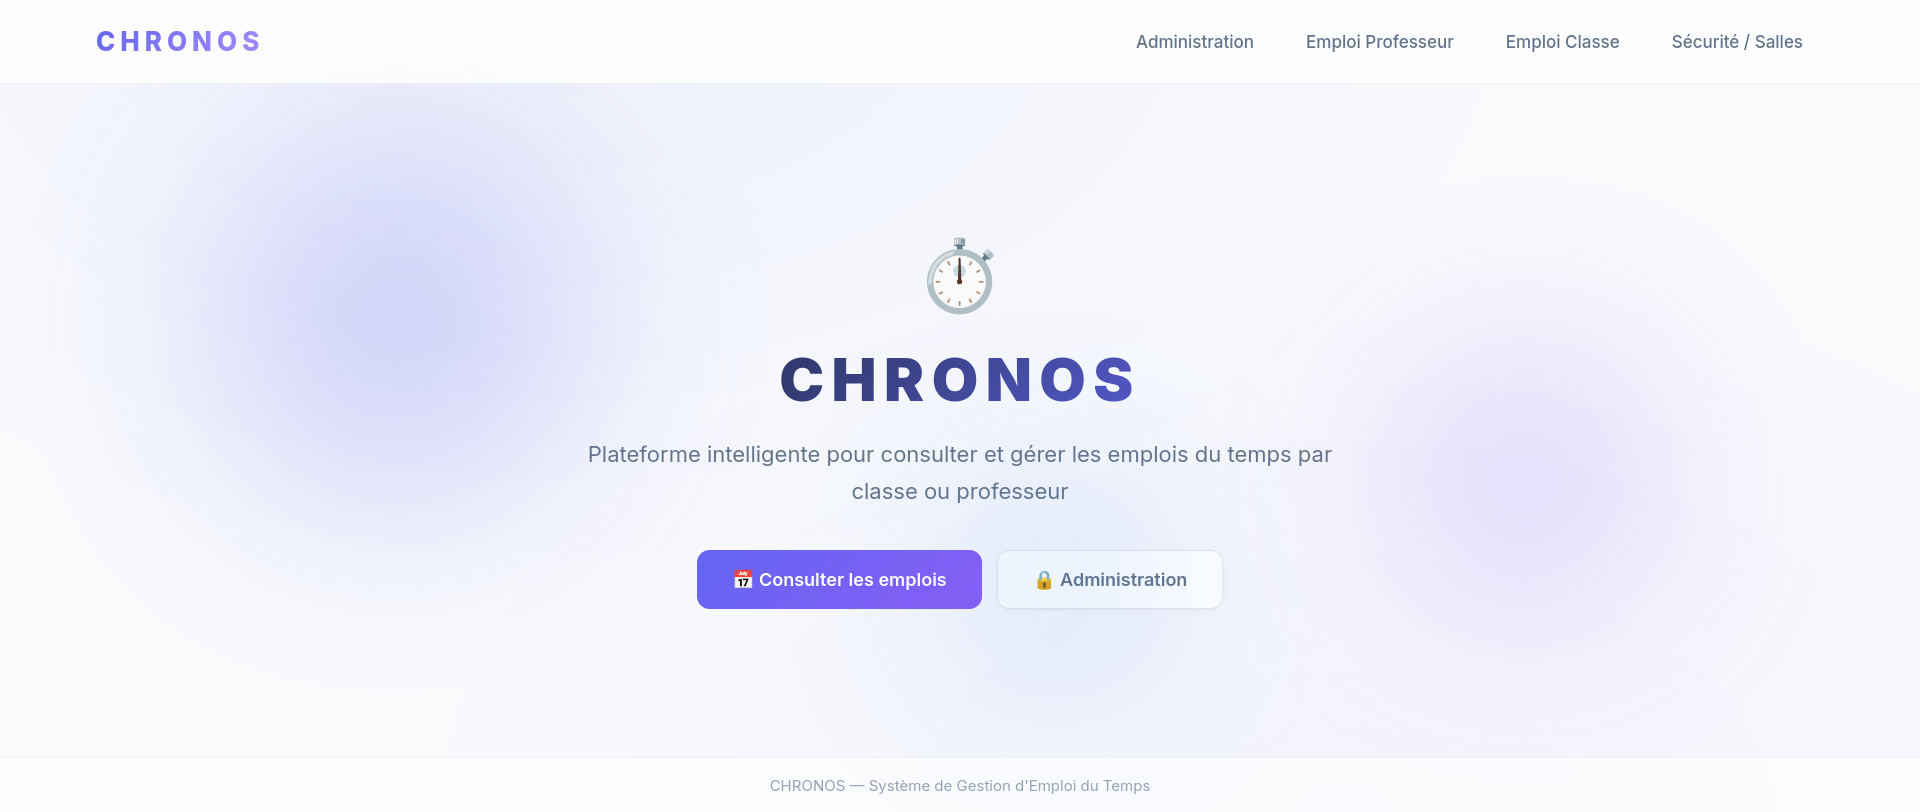
\includegraphics[width=\textwidth]{screens/Web/home.png}
    \caption{Page d'accueil du portail web Chronos. Elle sert de point d'entrée permettant l'accès aux différentes interfaces selon le rôle de l'utilisateur.}
\end{figure}

\subsection{Consultation de l'Emploi du Temps par Classe}

Cette vue permet à l'administrateur (ou à un étudiant via le portail) de visualiser la grille de cours assignée à une promotion spécifique (par exemple SIIA ou SMI). Le système interroge la table \texttt{EMPLOI\_DU\_TEMPS} en filtrant par \texttt{ID\_CLASSE}.

\begin{figure}[H]
    \centering
    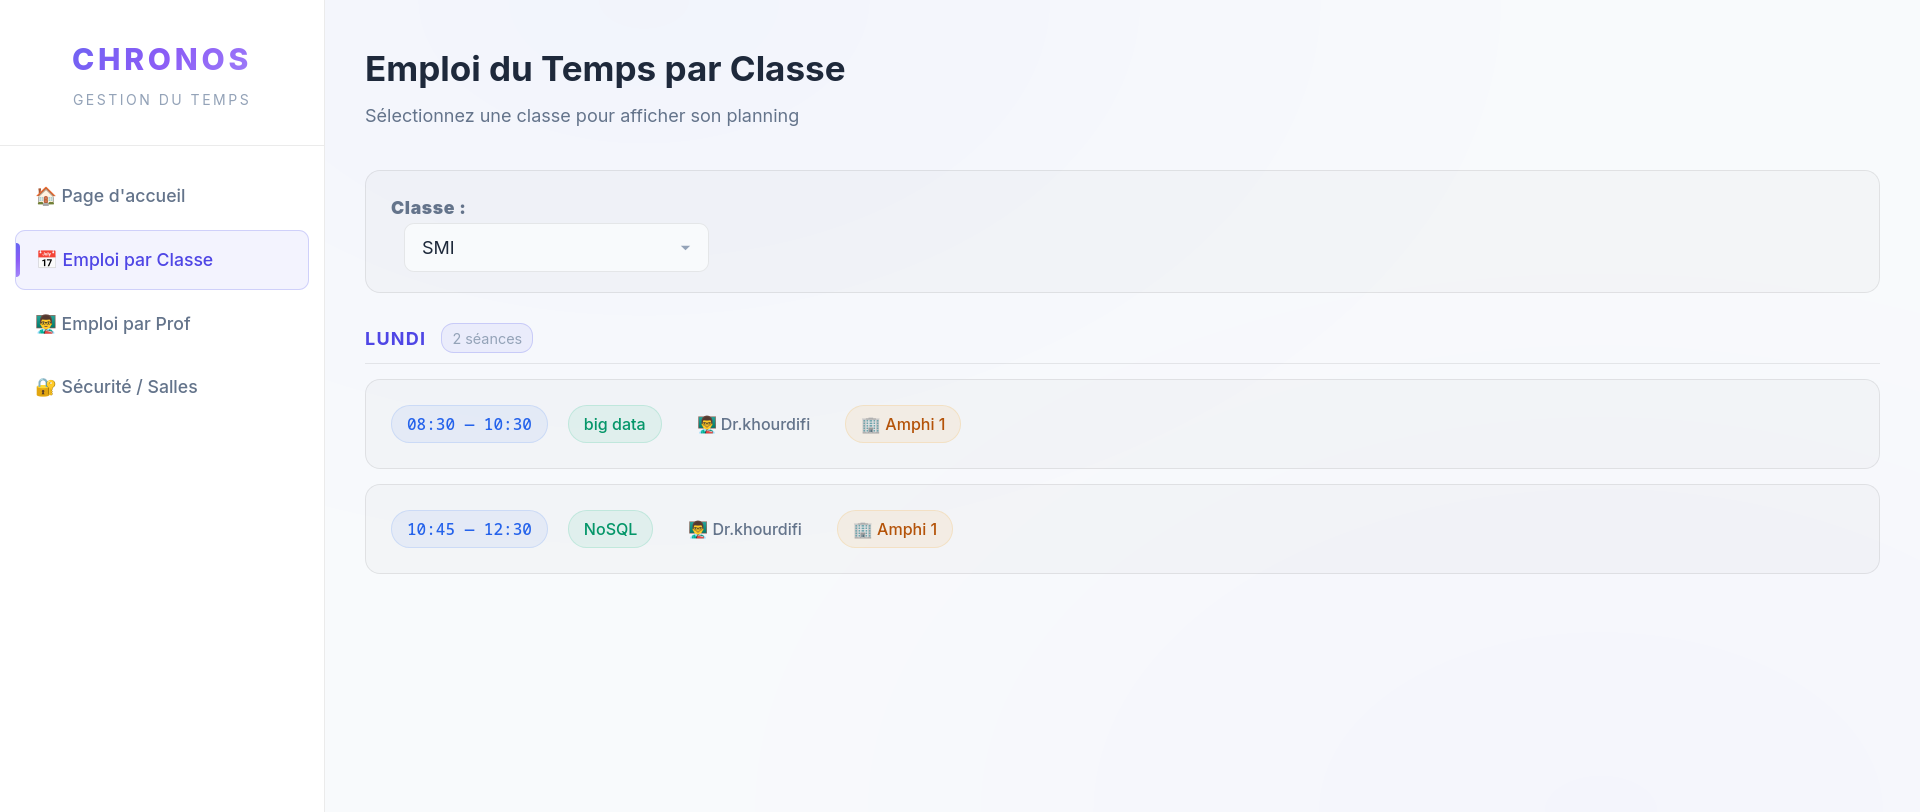
\includegraphics[width=\textwidth]{screens/Web/emploi_par_class.png}
    \caption{Emploi du temps affiché par classe. L'administrateur peut vérifier l'ensemble des cours assignés à une promotion donnée.}
\end{figure}

\subsection{Consultation de l'Emploi du Temps par Professeur}

De manière symétrique, cette interface filtre les séances par professeur (\texttt{ID\_PROF}), affichant les heures d'enseignement et les salles assignées pour chaque enseignant.

\begin{figure}[H]
    \centering
    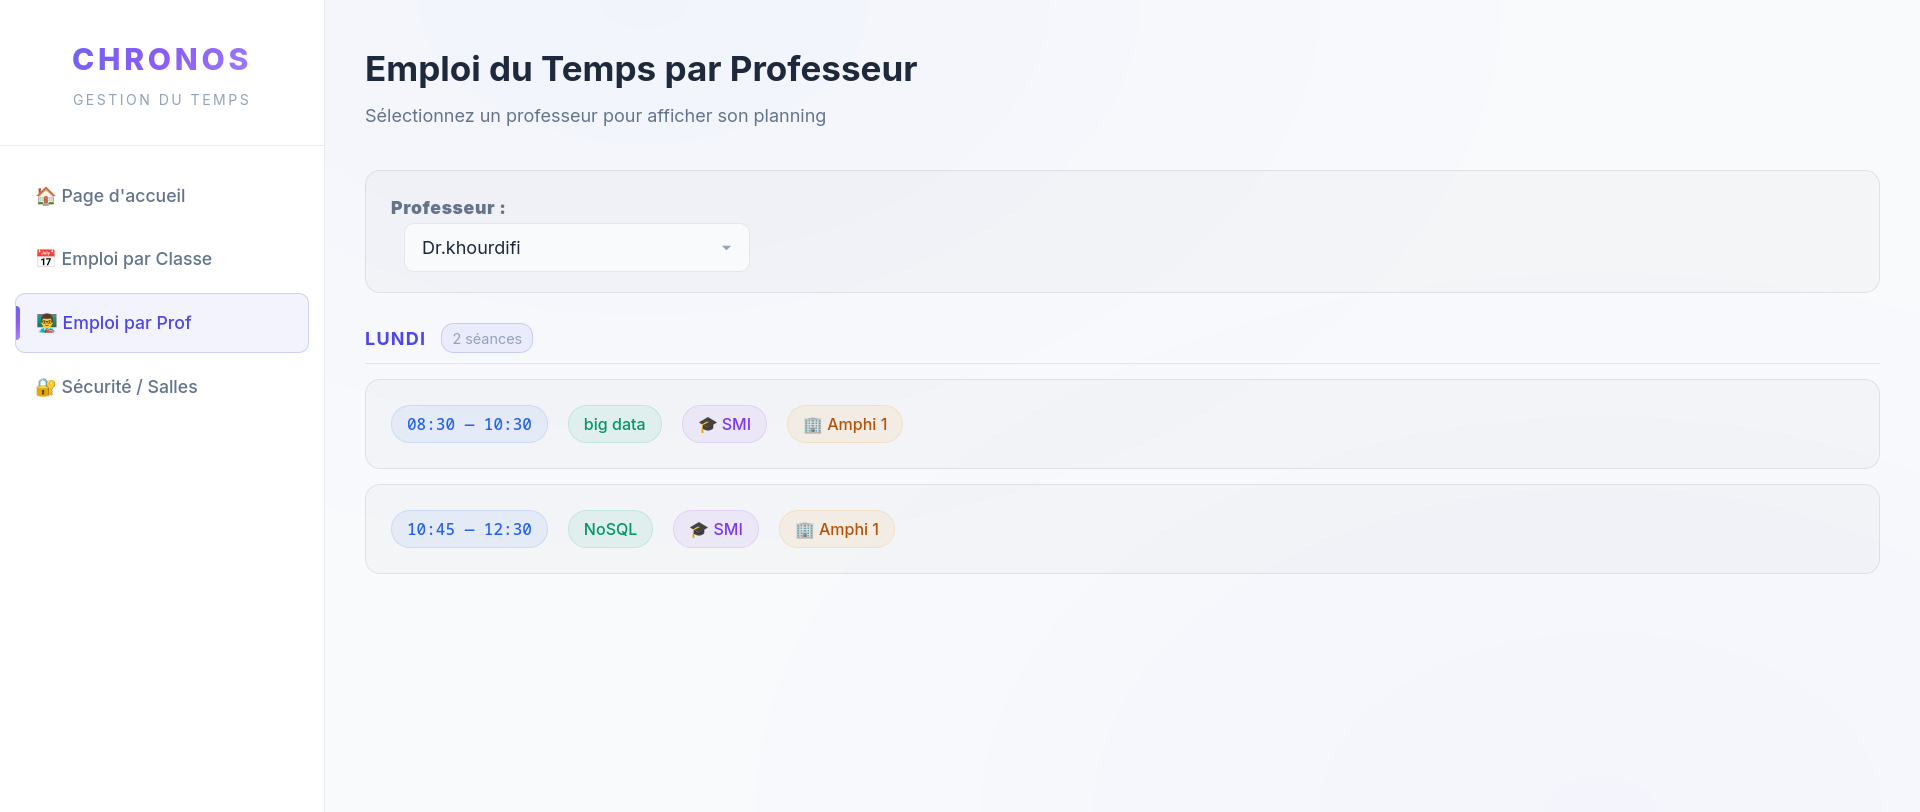
\includegraphics[width=\textwidth]{screens/Web/emploi_par_prof.png}
    \caption{Emploi du temps par professeur, montrant les créneaux horaires et les salles affectées à chaque enseignant.}
\end{figure}

\subsection{Vue Globale Sécurité}

Cette interface est conçue pour les agents de sécurité. Elle offre un aperçu global permettant de savoir quelles salles sont occupées à un instant donné, facilitant ainsi la gestion des accès et la surveillance du campus.

\begin{figure}[H]
    \centering
    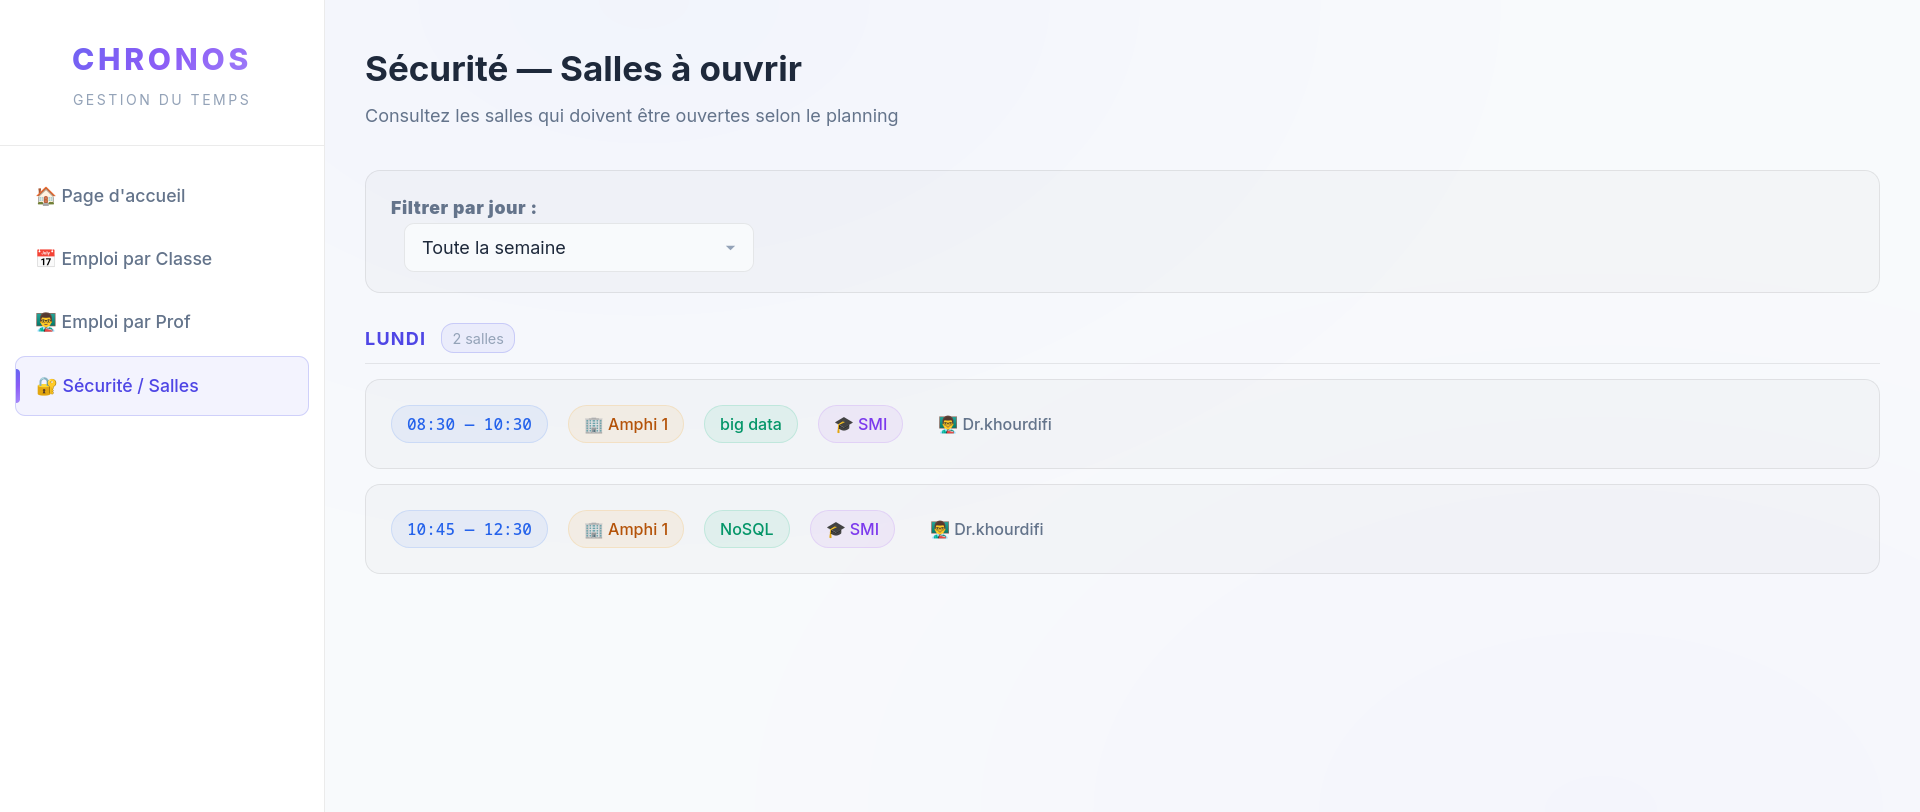
\includegraphics[width=\textwidth]{screens/Web/emploi_securite.png}
    \caption{Vue sécurité : aperçu global de l'occupation des salles pour les agents de sécurité du campus.}
\end{figure}

\subsection{Tableau de Bord Administrateur}

Le tableau de bord est le centre de contrôle principal de l'administrateur. Depuis cette interface, il peut accéder à toutes les opérations CRUD (Créer, Lire, Mettre à jour, Supprimer) sur les séances de cours, ainsi qu'à l'éditeur de carte du campus.

\begin{figure}[H]
    \centering
    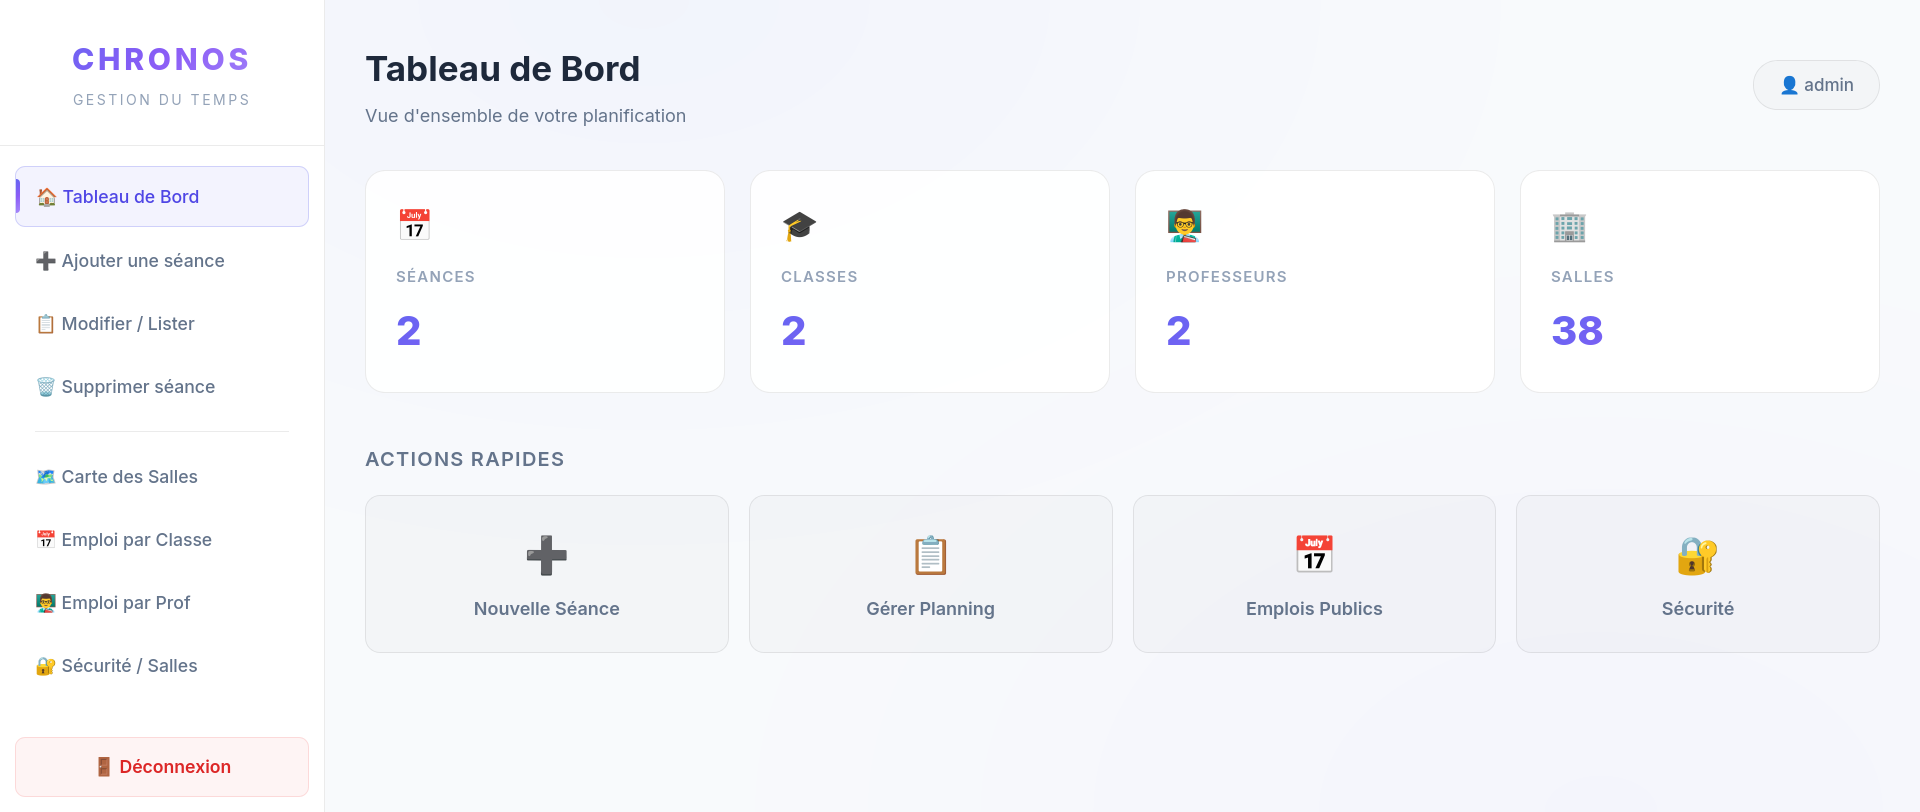
\includegraphics[width=\textwidth]{screens/Web/admin_dashboard.png}
    \caption{Tableau de bord de l'administrateur offrant l'accès aux fonctions de gestion des emplois du temps et de la carte.}
\end{figure}

\subsection{Ajout d'une Séance de Cours}

Le processus d'ajout d'une nouvelle séance se fait en plusieurs étapes via des formulaires interactifs. L'administrateur sélectionne le professeur, le cours, la classe, la salle et le créneau horaire. Le système vérifie la disponibilité de la salle afin d'éviter tout conflit d'emploi du temps.

\begin{figure}[H]
    \centering
    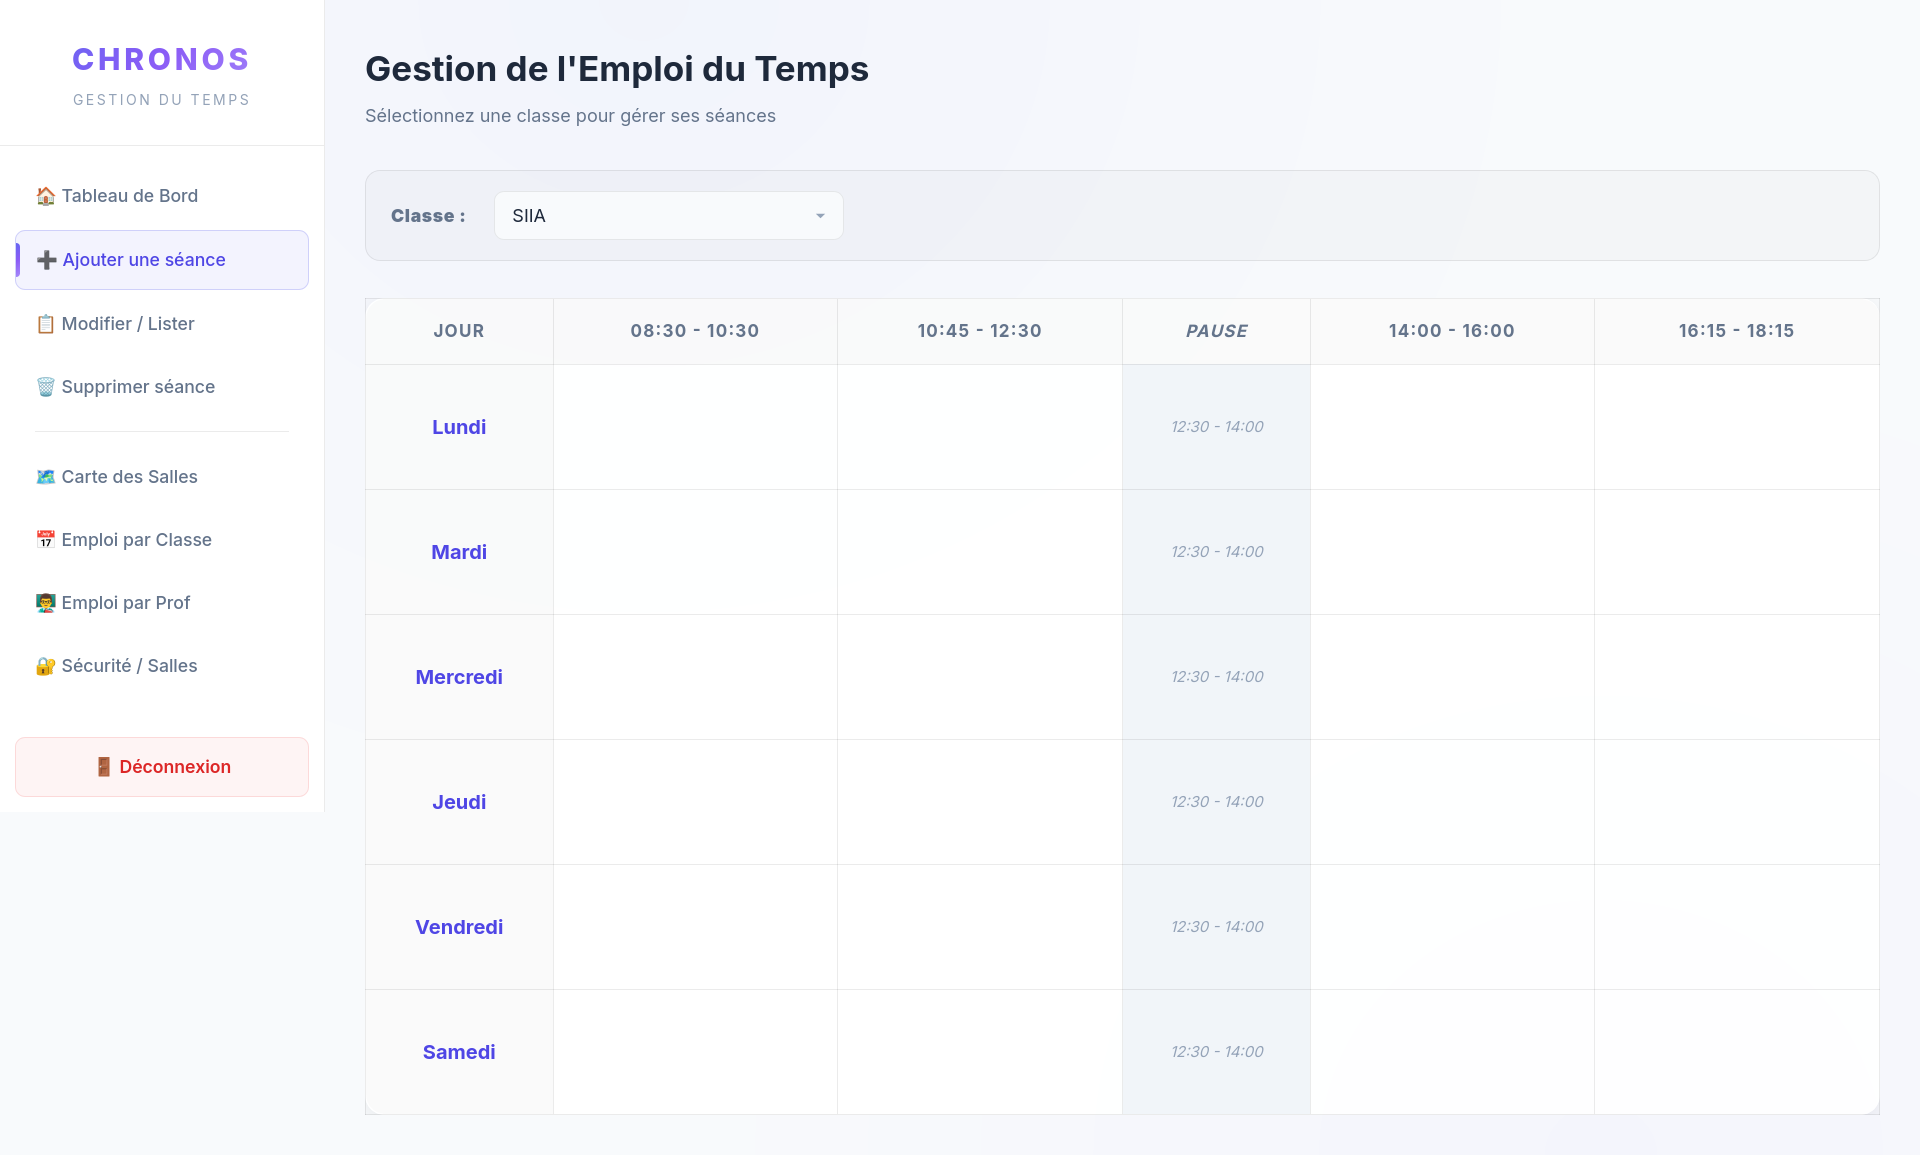
\includegraphics[width=\textwidth]{screens/Web/admin_add_seance1.png}
    \caption{Ajout d'une séance -- Étape 1 : sélection du professeur, du cours et de la classe cible.}
\end{figure}

\begin{figure}[H]
    \centering
    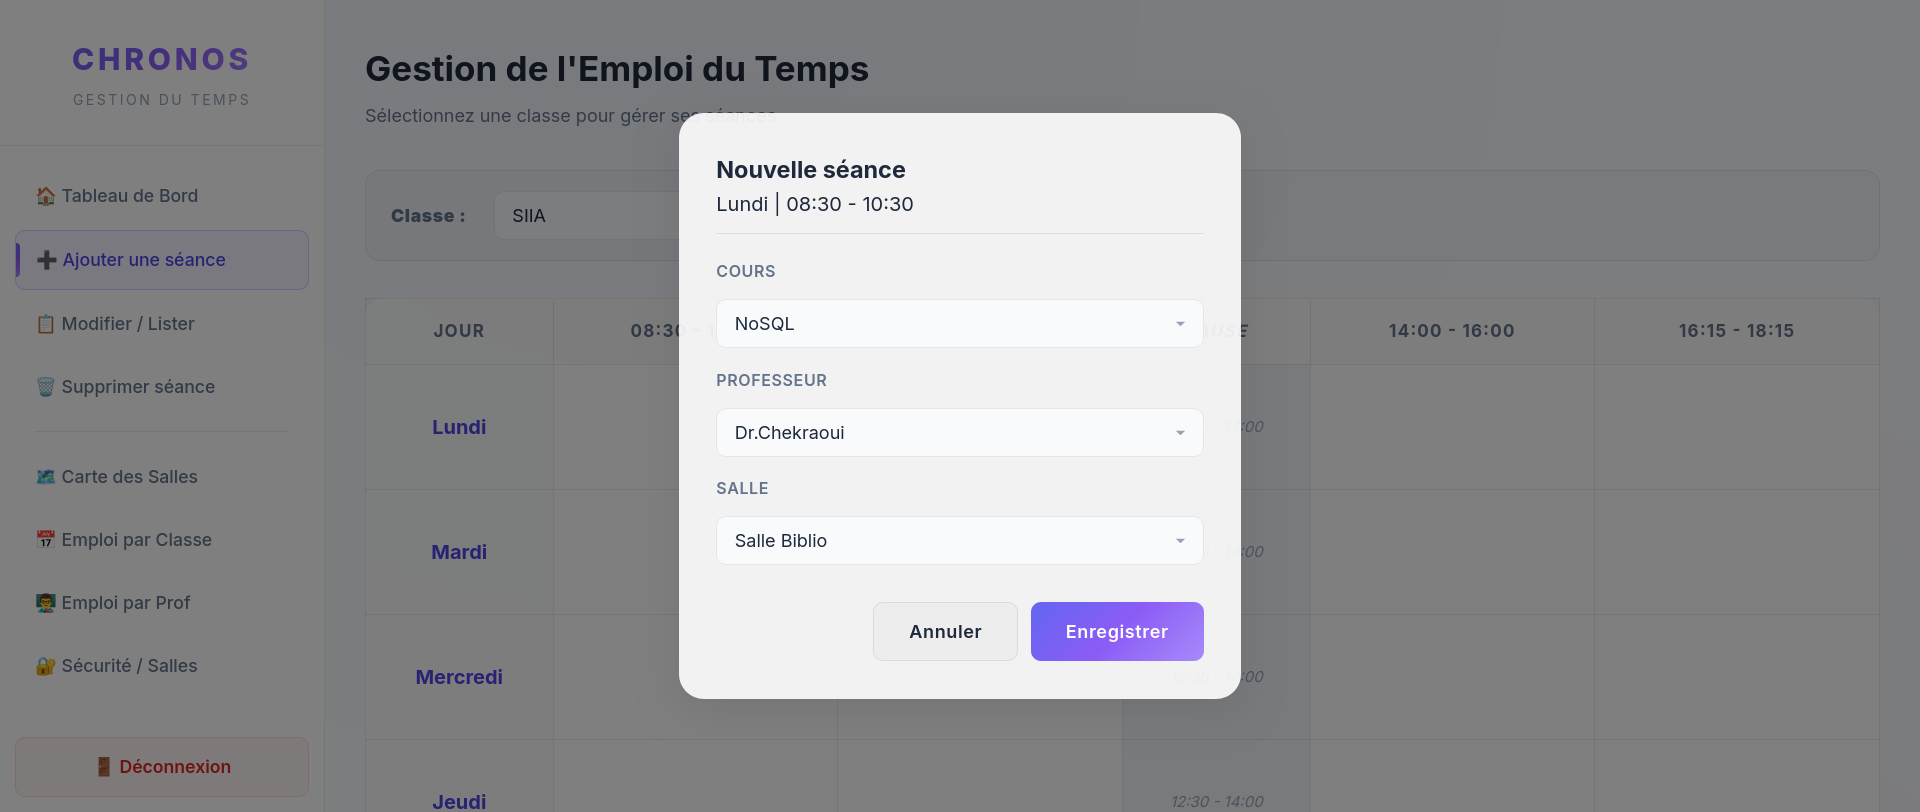
\includegraphics[width=\textwidth]{screens/Web/admin_add_seance2.png}
    \caption{Ajout d'une séance -- Étape 2 : choix de la salle et du créneau horaire avec vérification de disponibilité.}
\end{figure}

\subsection{Liste et Modification des Séances}

L'administrateur peut consulter la liste complète de toutes les séances existantes dans la base de données. Depuis cette liste, il peut sélectionner une séance pour la modifier (changement de salle, d'horaire, de professeur) ou la supprimer.

\begin{figure}[H]
    \centering
    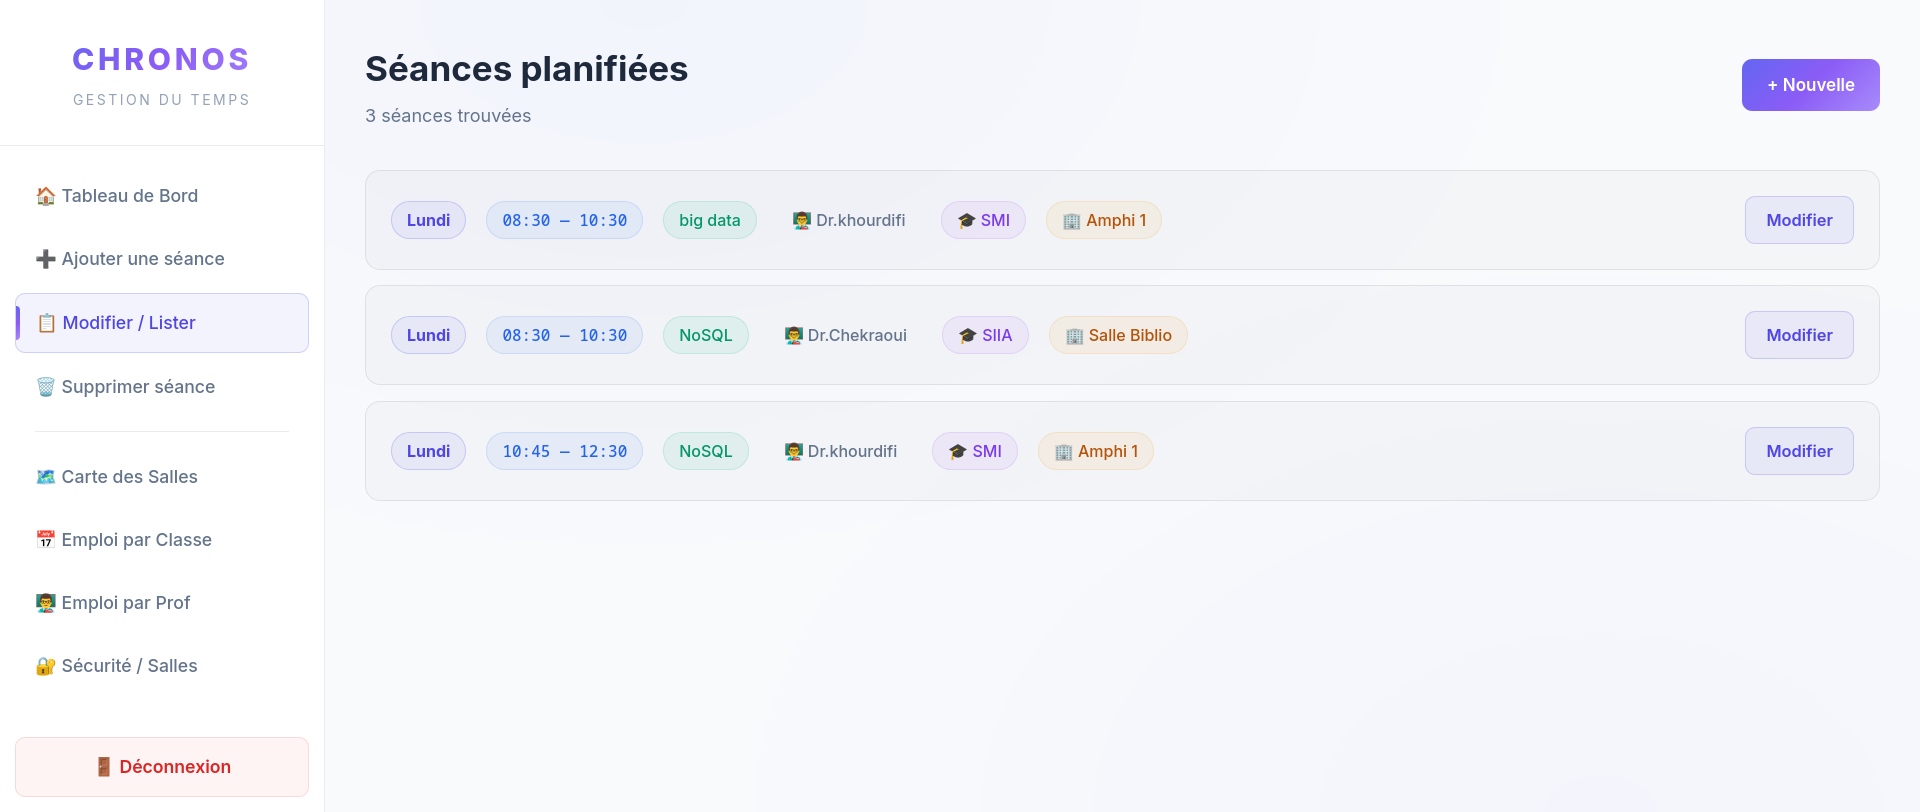
\includegraphics[width=\textwidth]{screens/Web/admin_modify_list.png}
    \caption{Liste complète des séances enregistrées, avec options de modification et de suppression.}
\end{figure}

\begin{figure}[H]
    \centering
    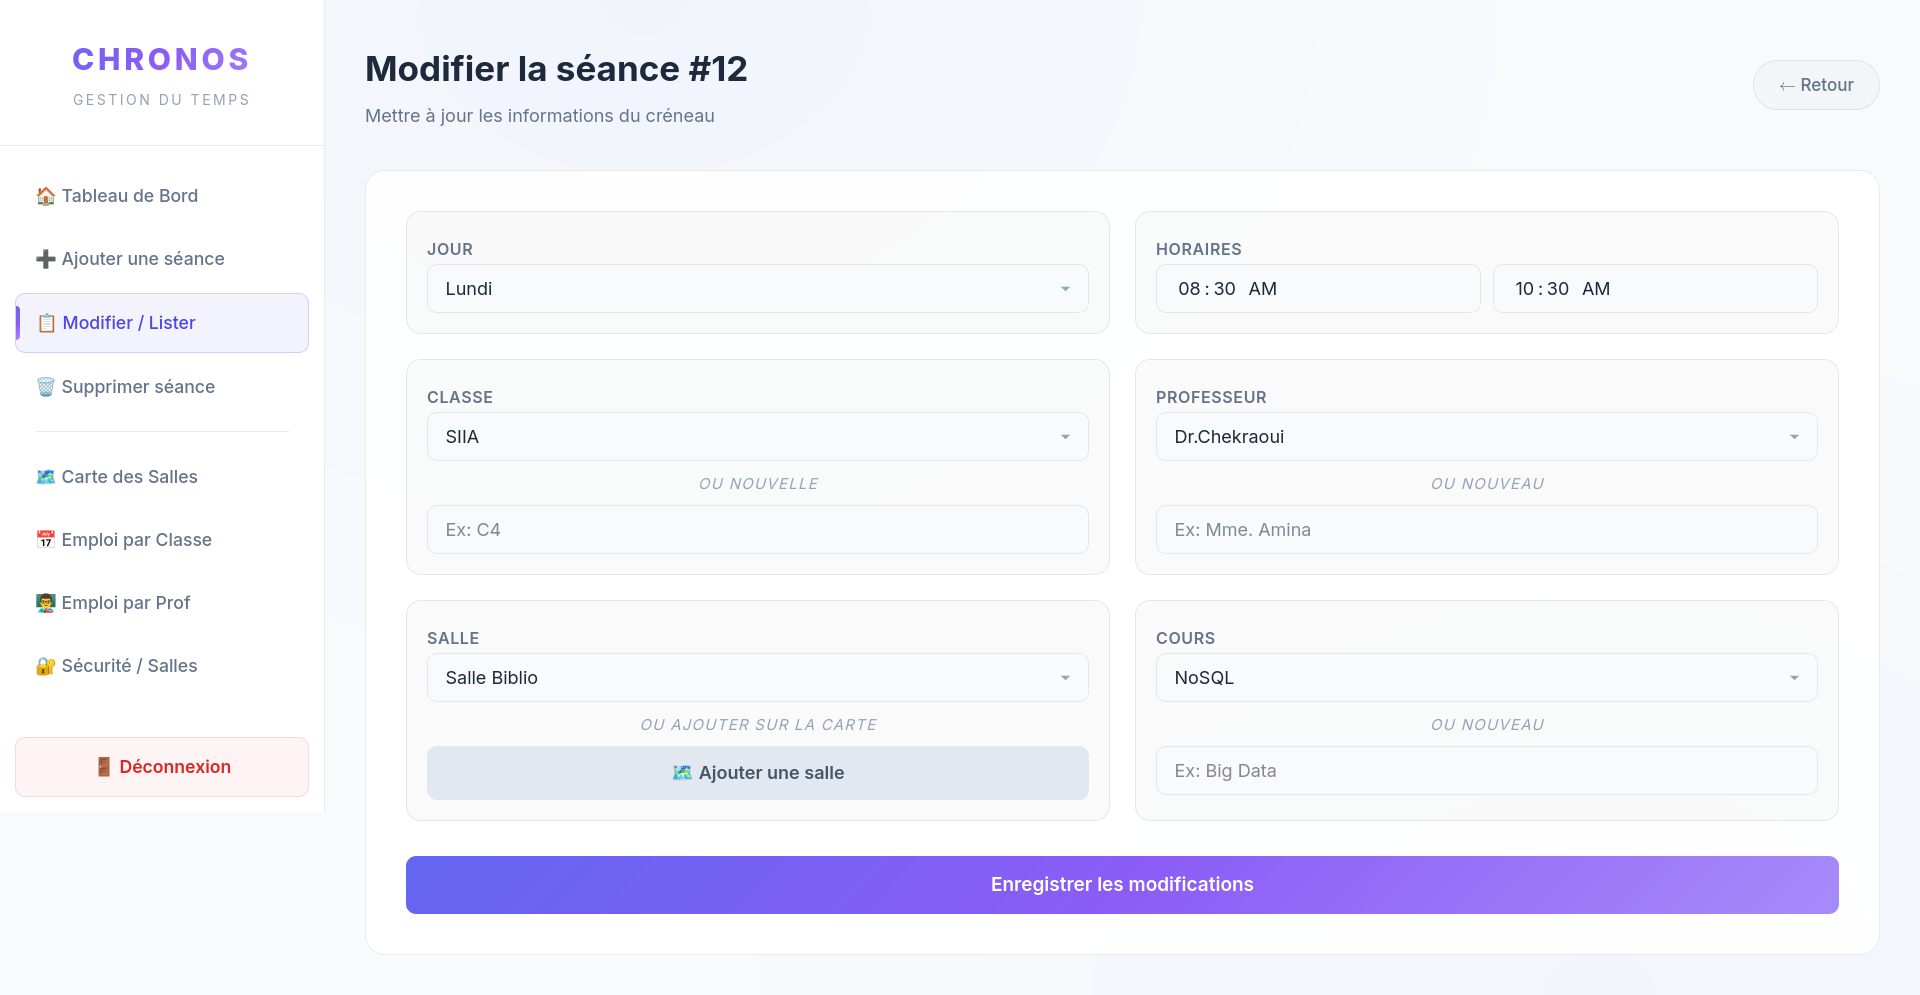
\includegraphics[width=\textwidth]{screens/Web/admin_modify.png}
    \caption{Interface de modification d'une séance existante : changement du créneau, de la salle ou du professeur en temps réel.}
\end{figure}

\subsection{Suppression d'une Séance}

La suppression d'une séance est gérée par le fichier \texttt{delete\_et.php}. Après confirmation, la séance est retirée de la table \texttt{EMPLOI\_DU\_TEMPS}, et les changements sont immédiatement répercutés sur l'application mobile via l'API.

\begin{figure}[H]
    \centering
    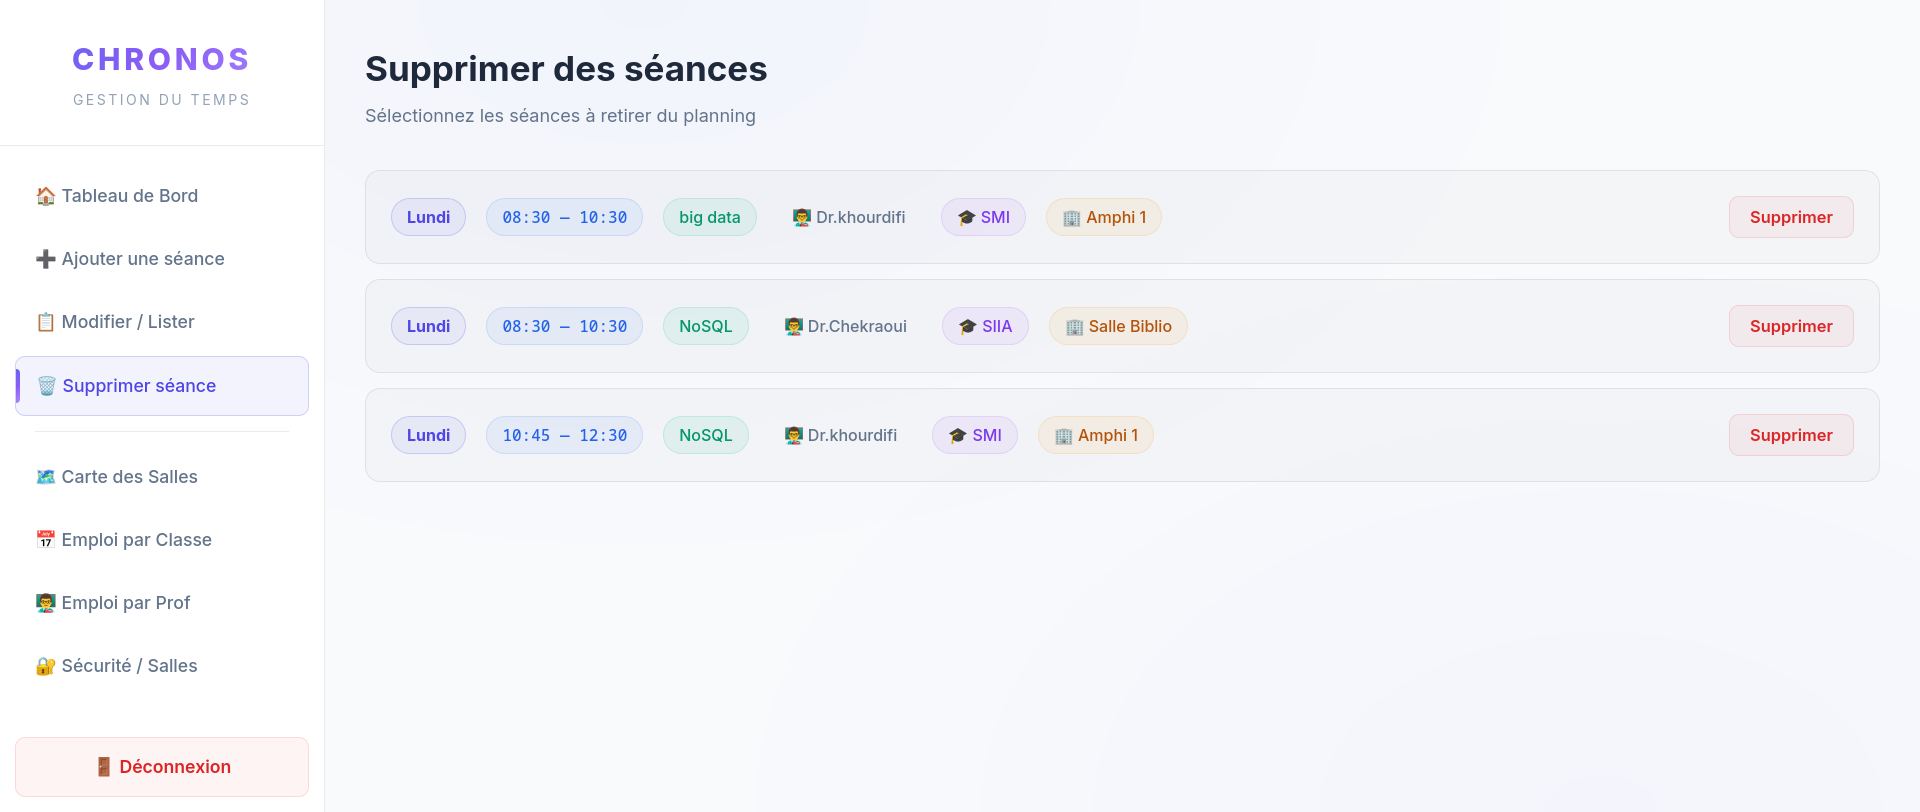
\includegraphics[width=\textwidth]{screens/Web/admin_supprimer_seance.png}
    \caption{Interface de suppression d'une séance avec confirmation, assurant une propagation instantanée vers le mobile.}
\end{figure}

\subsection{Éditeur de Carte Interactive du Campus}

C'est la \textbf{fonctionnalité la plus novatrice} du projet. L'administrateur peut littéralement \textbf{dessiner} l'agencement du campus sur une grille interactive. Il place des cellules de type \texttt{classroom} (salle), \texttt{road} (route), ou \texttt{entrance} (entrée) directement sur la grille. Le résultat est sérialisé en JSON et stocké dans la table \texttt{CARTE\_LAYOUT}. Ce JSON est ensuite récupéré en temps réel par l'application mobile, qui le parse pour construire dynamiquement une carte tactile navigable.

\begin{figure}[H]
    \centering
    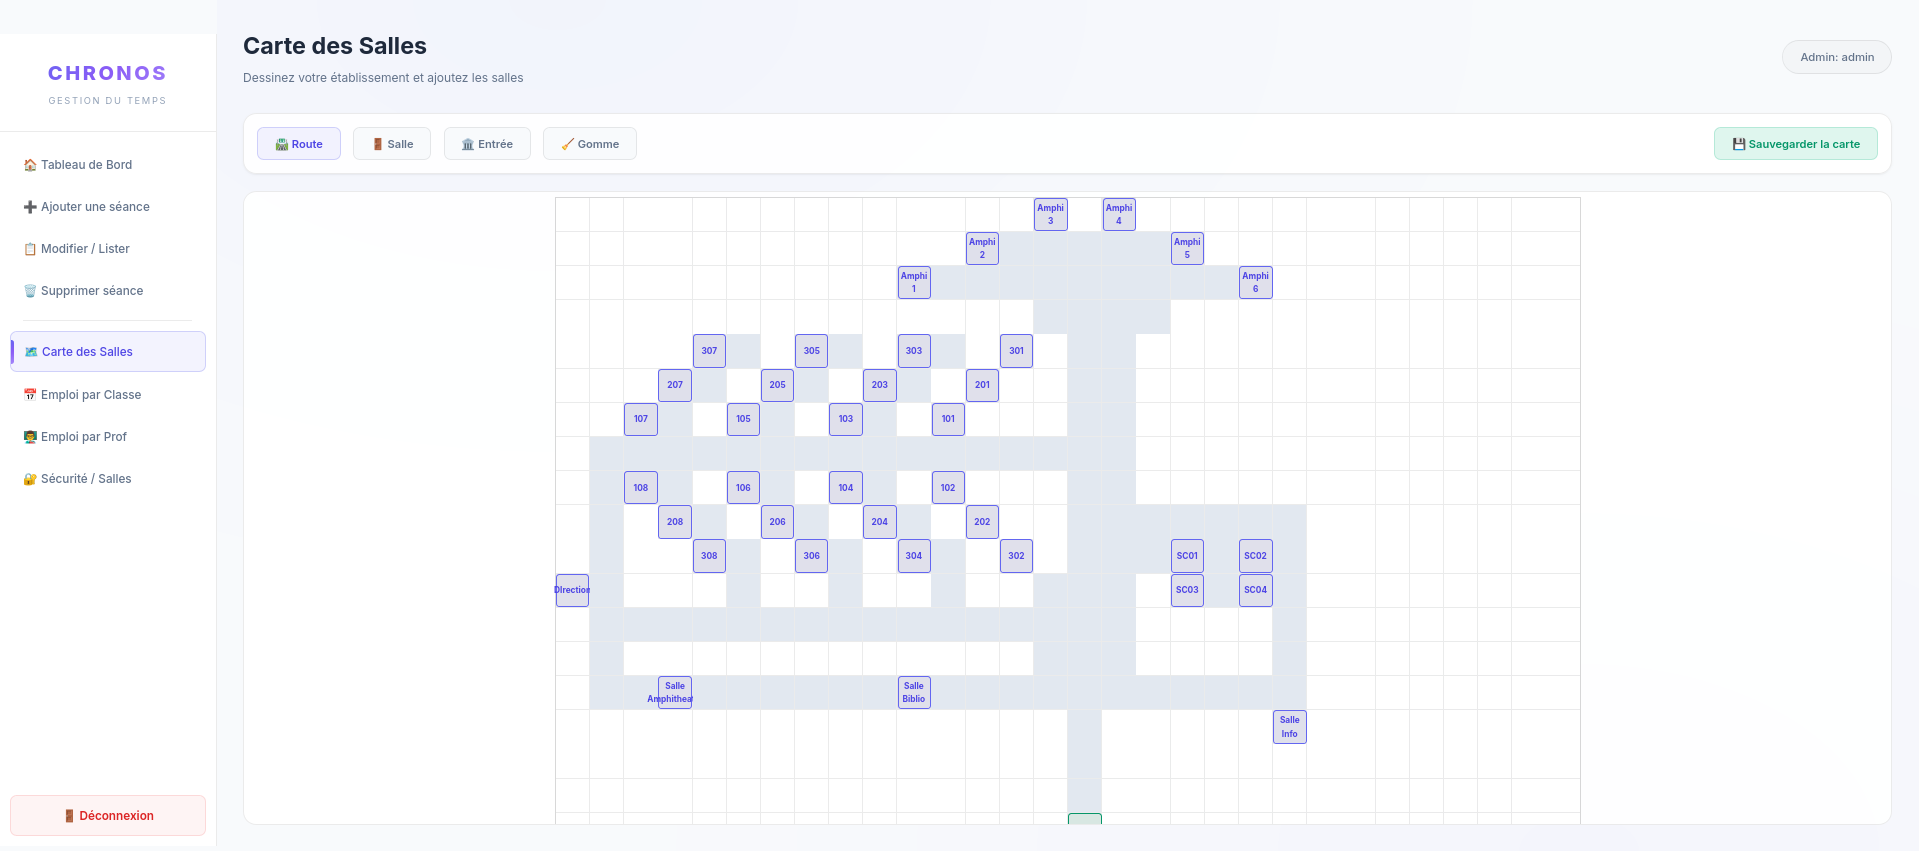
\includegraphics[width=\textwidth]{screens/Web/admin_map.png}
    \caption{Éditeur de carte interactive : l'administrateur dessine les bâtiments, les routes et les entrées du campus sur une grille.}
\end{figure}


% ============================================================
% CHAPITRE 5 : L'APPLICATION MOBILE
% ============================================================
\chapter{L'Application Mobile : Dédiée aux Utilisateurs}

\section{Présentation Générale}

Contrairement au portail web qui est réservé à l'administration, l'application mobile Chronos est \textbf{spécifiquement conçue pour les utilisateurs finaux} : les étudiants, les professeurs et les agents de sécurité. Son objectif est de leur offrir un accès nomade, fluide et en temps réel à leur emploi du temps et à la carte interactive du campus.

L'application a été développée avec le framework \textbf{Flutter} (langage Dart), ce qui la rend \textbf{multiplateforme} : elle est compilable pour Android (\texttt{.apk}), iOS, ou même en version Web exécutable dans un navigateur.

\textbf{Point clé :} L'application est \textbf{100\% côté client} (client-side). Elle ne contient aucune base de données locale complexe. Elle consomme exclusivement les données fournies par l'API REST hébergée sur Alwaysdata.

\section{Structure du Code Flutter}

\begin{table}[H]
\centering
\renewcommand{\arraystretch}{1.3}
\begin{tabularx}{\textwidth}{l X}
\toprule
\textbf{Fichier / Répertoire} & \textbf{Rôle} \\
\midrule
\texttt{lib/main.dart} & Point d'entrée de l'application, configuration du routeur \\
\texttt{lib/login\_page.dart} & Écran de connexion \\
\texttt{lib/models/user.dart} & Modèle Dart de l'utilisateur (\texttt{User.fromJson()}) \\
\texttt{lib/models/session.dart} & Modèle Dart d'une séance de cours \\
\texttt{lib/services/api\_service.dart} & Client HTTP central (GET, POST, gestion du Bearer Token) \\
\texttt{lib/services/auth\_service.dart} & Gestion de l'authentification \\
\texttt{lib/services/timetable\_service.dart} & Récupération des emplois du temps \\
\texttt{lib/services/map\_service.dart} & Récupération des données de la carte \\
\texttt{lib/screens/dashboard\_screen.dart} & Tableau de bord étudiant \\
\texttt{lib/screens/professor\_dashboard\_screen.dart} & Tableau de bord professeur \\
\texttt{lib/screens/security\_dashboard\_screen.dart} & Tableau de bord sécurité \\
\texttt{lib/screens/map\_view.dart} & Rendu interactif de la carte du campus \\
\bottomrule
\end{tabularx}
\caption{Structure du code source de l'application mobile Flutter.}
\end{table}

\section{Écrans de l'Application Mobile}

\subsection{Écran de Connexion}

L'application démarre sur un écran de connexion sécurisé. L'utilisateur saisit ses identifiants (email et mot de passe). Le service \texttt{auth\_service.dart} envoie ces données à l'API REST. Si l'authentification réussit, un jeton Bearer Token est renvoyé et stocké en mémoire via \texttt{ApiService.setAuthToken()}. Toutes les requêtes suivantes incluent automatiquement ce jeton dans l'en-tête \texttt{Authorization}.

\begin{figure}[H]
    \centering
    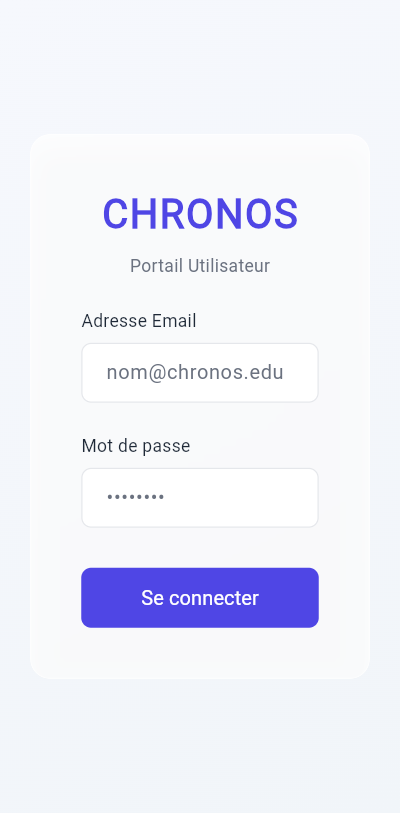
\includegraphics[width=0.4\textwidth]{screens/Mobile/login.png}
    \caption{Écran de connexion mobile. L'utilisateur (étudiant, professeur ou agent de sécurité) saisit ses identifiants pour accéder à ses données.}
\end{figure}

\subsection{Profil Utilisateur}

Après connexion, l'utilisateur peut consulter son profil, qui affiche son nom complet, son email, son rôle (\texttt{student}, \texttt{professor}, \texttt{security}) et, pour les étudiants, sa classe d'appartenance.

\begin{figure}[H]
    \centering
    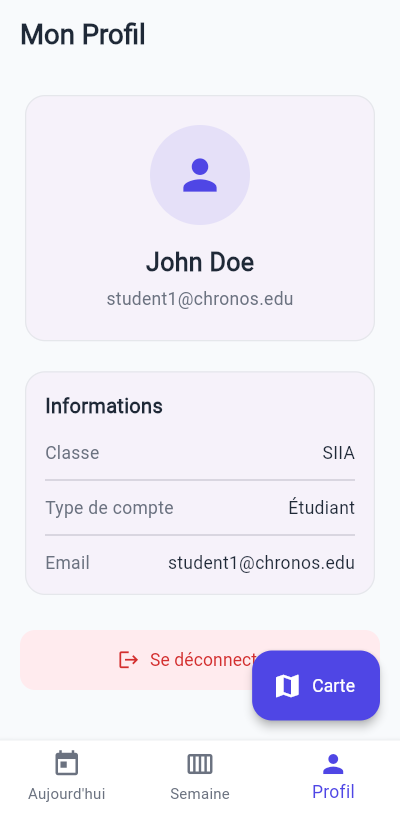
\includegraphics[width=0.4\textwidth]{screens/Mobile/profile.png}
    \caption{Profil de l'utilisateur connecté, affichant ses informations personnelles et son rôle dans le système.}
\end{figure}

\subsection{Emploi du Temps -- Vue par Jour}

L'écran principal de l'application affiche l'emploi du temps de la journée en cours. Pour chaque séance, le modèle \texttt{Session} affiche le nom du cours, le professeur, la salle et la plage horaire formatée (ex : \texttt{08:30 - 12:30}).

\begin{figure}[H]
    \centering
    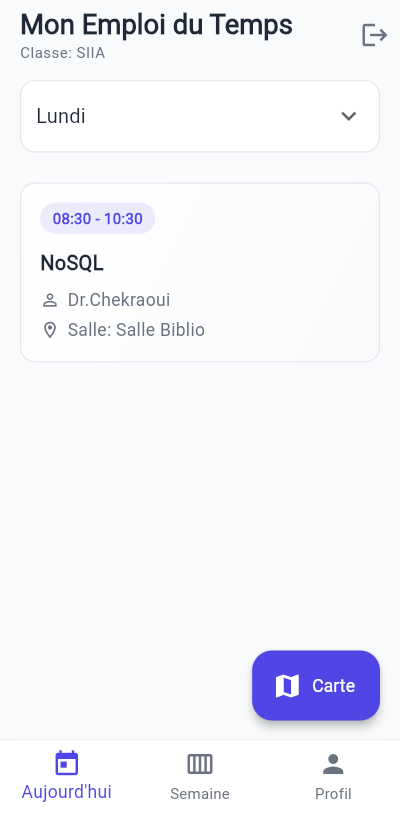
\includegraphics[width=0.4\textwidth]{screens/Mobile/day_view.png}
    \caption{Vue journalière de l'emploi du temps, récupérée en temps réel depuis l'API. Chaque séance affiche le cours, le professeur, la salle et l'horaire.}
\end{figure}

\subsection{Emploi du Temps -- Vue par Semaine}

Une vue hebdomadaire permet à l'utilisateur de visualiser l'ensemble de ses cours sur la semaine, facilitant l'organisation de son planning et l'anticipation de ses déplacements.

\begin{figure}[H]
    \centering
    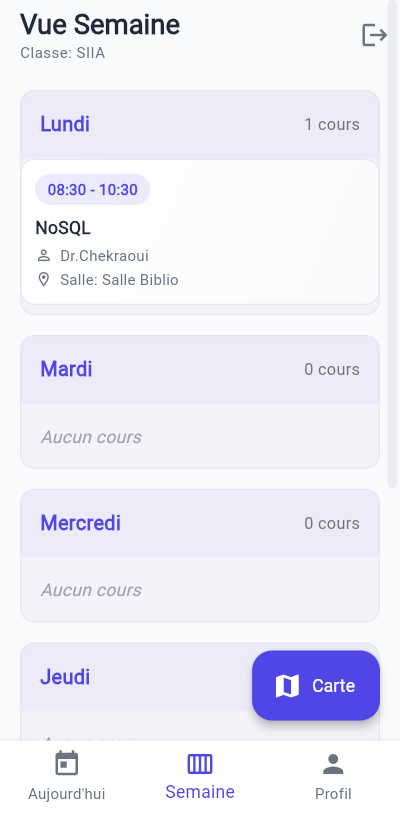
\includegraphics[width=0.4\textwidth]{screens/Mobile/week_view.png}
    \caption{Vue hebdomadaire offrant un aperçu complet de tous les cours de la semaine pour mieux planifier ses journées.}
\end{figure}

\subsection{Carte Interactive du Campus}

La carte interactive est la fonctionnalité phare de l'application mobile. Le service \texttt{map\_service.dart} récupère le JSON de la table \texttt{CARTE\_LAYOUT} via l'API, et l'écran \texttt{map\_view.dart} reconstruit dynamiquement une grille tactile où chaque cellule est colorée selon son type :

\begin{itemize}
    \item \textbf{Bleu} pour les salles de classe (\texttt{classroom}) avec leur nom affiché.
    \item \textbf{Gris} pour les routes (\texttt{road}).
    \item \textbf{Vert} pour les entrées (\texttt{entrance}).
    \item \textbf{Blanc/transparent} pour les espaces vides (\texttt{empty}).
\end{itemize}

L'utilisateur peut naviguer sur cette carte de manière fluide grâce aux gestes tactiles (zoom, défilement).

\begin{figure}[H]
    \centering
    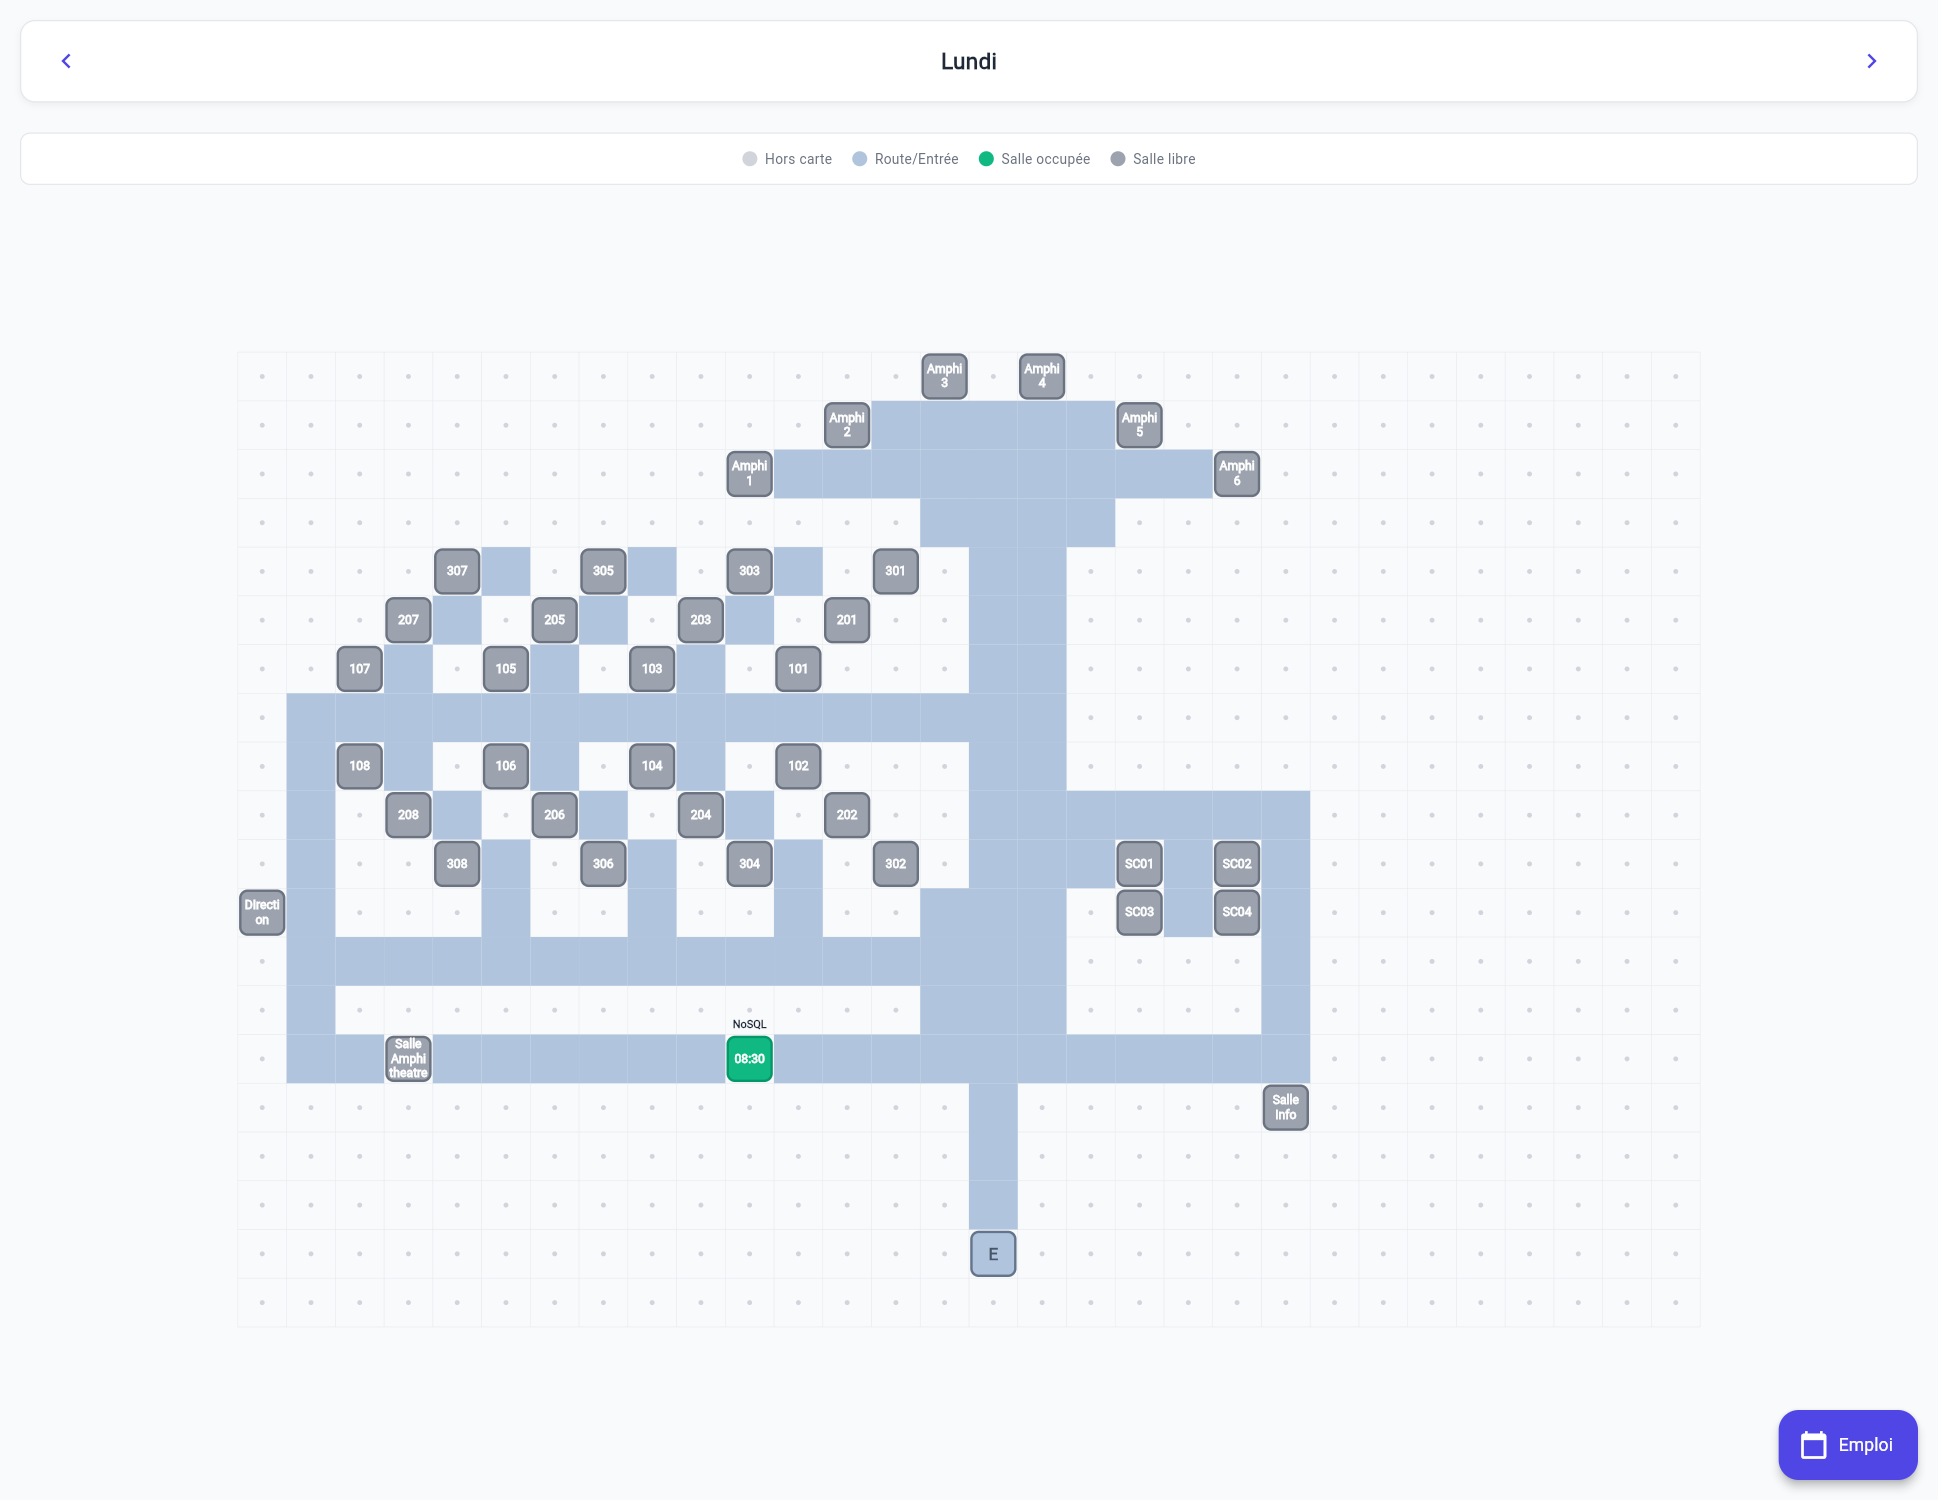
\includegraphics[width=0.55\textwidth]{screens/Mobile/map_view1.png}
    \caption{Carte interactive du campus (Vue 1). Générée dynamiquement à partir du dessin de l'administrateur, elle permet aux étudiants de s'orienter facilement.}
\end{figure}

\begin{figure}[H]
    \centering
    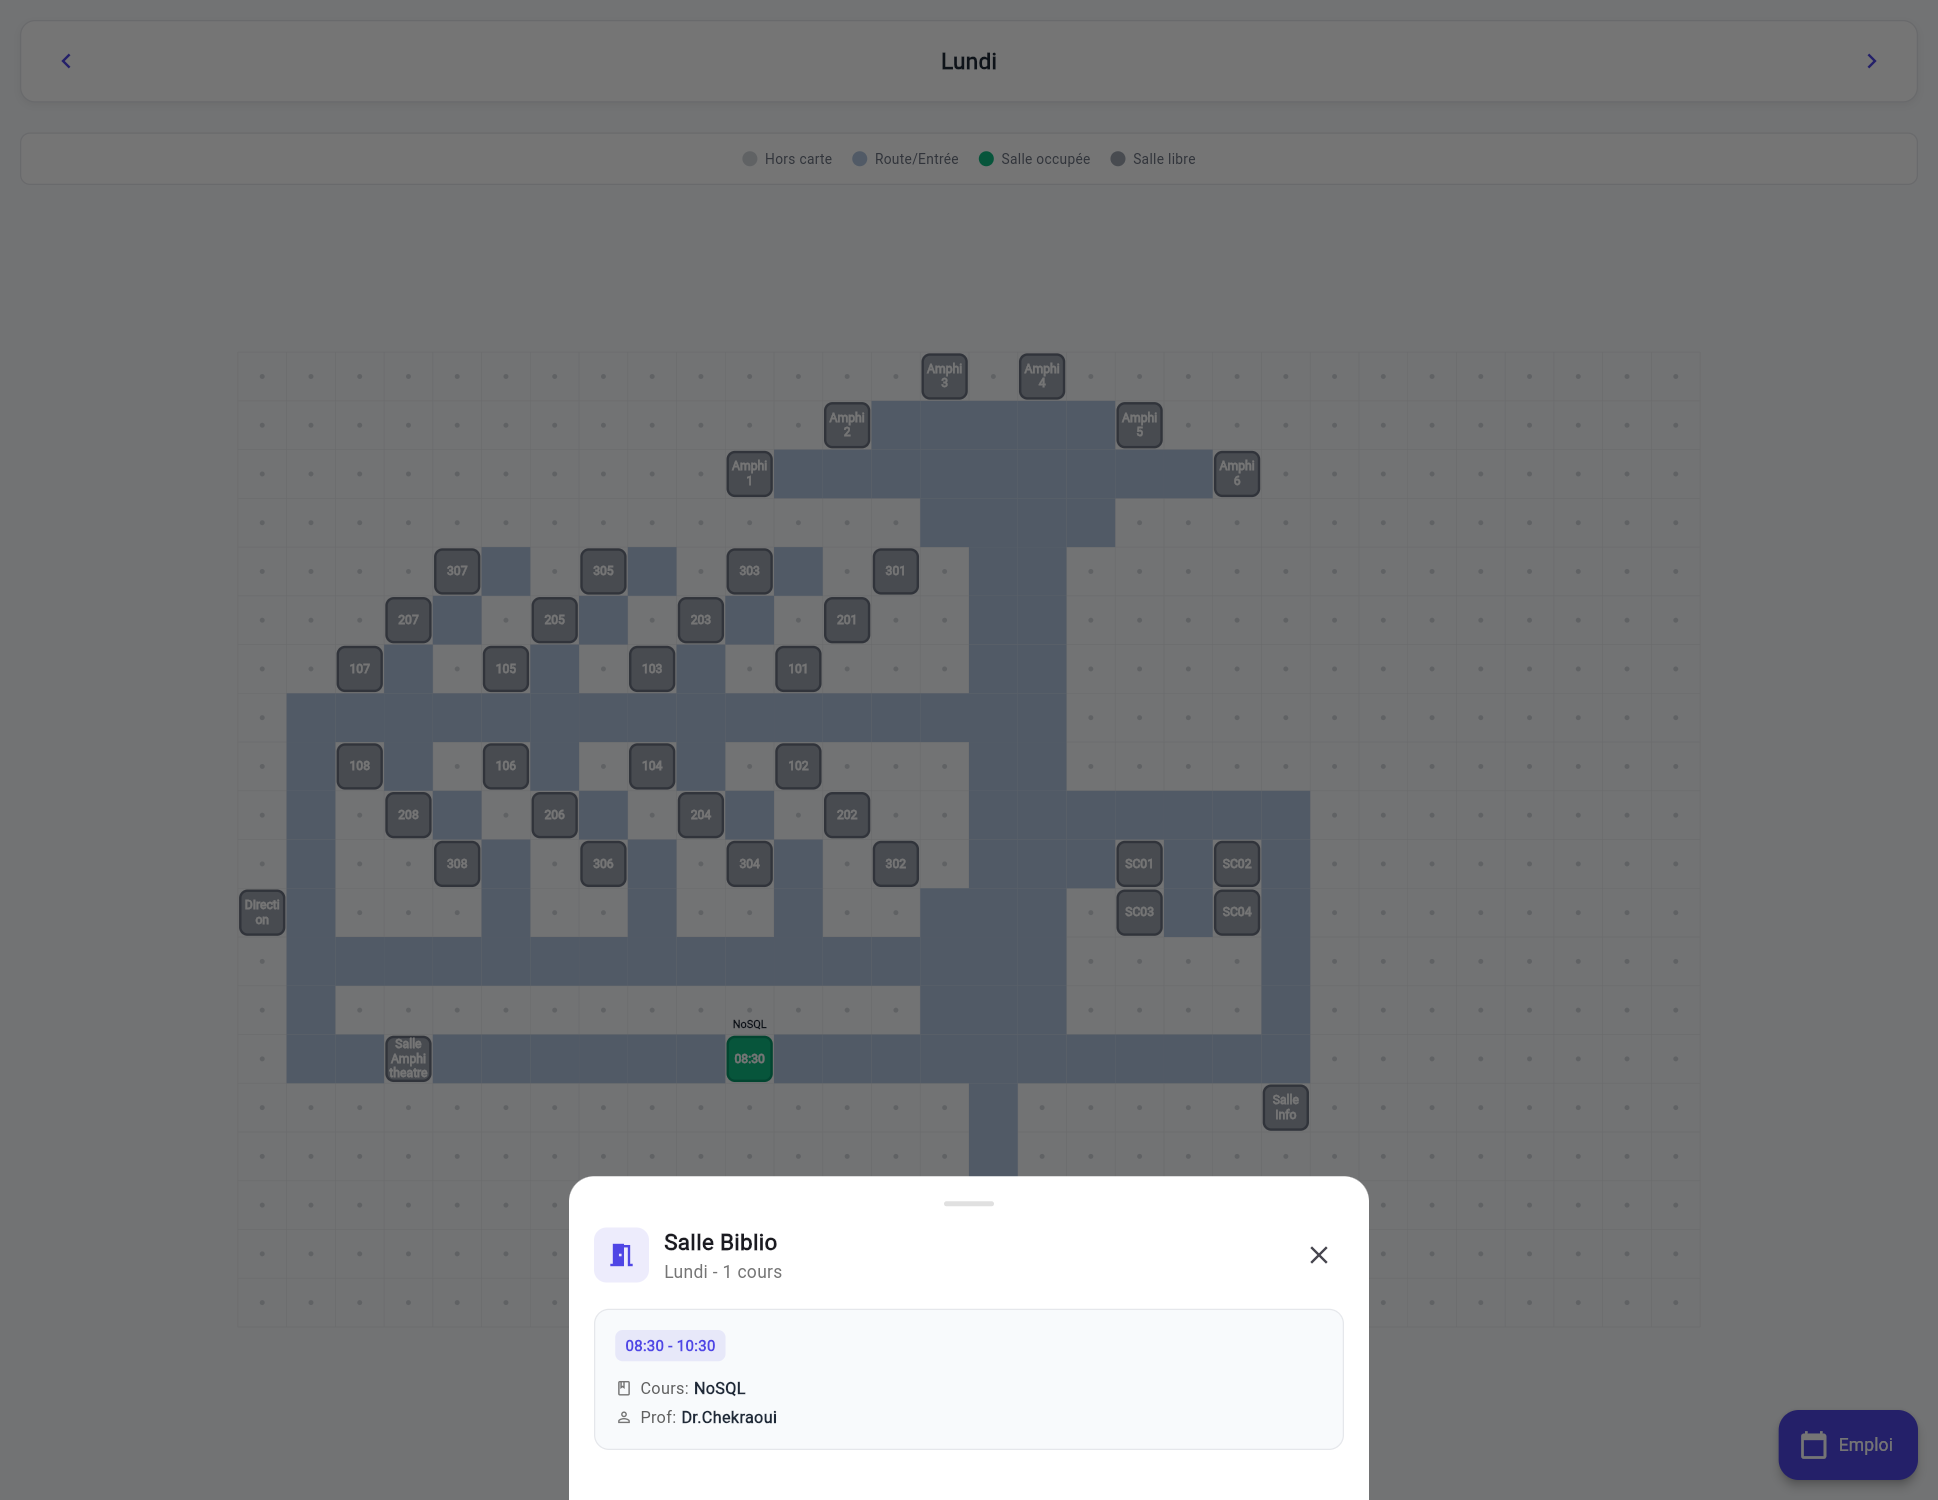
\includegraphics[width=0.55\textwidth]{screens/Mobile/map_view2.png}
    \caption{Carte interactive du campus (Vue 2). L'utilisateur peut explorer les salles spécifiques (Salle Info, Salle Biblio, SC01) via cette interface tactile.}
\end{figure}


% ============================================================
% CHAPITRE 6 : L'API REST
% ============================================================
\chapter{L'API REST : Le Pont entre Web et Mobile}

\section{Rôle de l'API}

L'API REST est le \textbf{c\oe{}ur de la communication} entre le portail d'administration web et l'application mobile. Elle est développée en PHP et déployée dans le répertoire \texttt{api/} sur le serveur Alwaysdata.

Son rôle est triple :
\begin{enumerate}
    \item \textbf{Authentifier} les utilisateurs mobiles (vérification des identifiants et génération de jetons).
    \item \textbf{Servir} les données (emplois du temps, carte) au format JSON.
    \item \textbf{Sécuriser} les accès via la validation du Bearer Token à chaque requête.
\end{enumerate}

\section{Structure de l'API}

\begin{table}[H]
\centering
\renewcommand{\arraystretch}{1.3}
\begin{tabularx}{\textwidth}{l X}
\toprule
\textbf{Fichier} & \textbf{Rôle} \\
\midrule
\texttt{api/config.php} & Configuration CORS, connexion PDO, fonctions utilitaires (tokens) \\
\texttt{api/auth/} & Endpoints d'authentification (login, logout) \\
\texttt{api/student/} & Endpoints pour les données étudiants \\
\texttt{api/prof/} & Endpoints pour les données professeurs \\
\texttt{api/security/} & Endpoints pour les données sécurité \\
\texttt{api/map/} & Endpoint pour récupérer la carte du campus \\
\bottomrule
\end{tabularx}
\caption{Structure des endpoints de l'API REST.}
\end{table}

\section{Mécanisme d'Authentification}

Le mécanisme d'authentification repose sur un système de \textbf{Bearer Token} :

\begin{enumerate}
    \item L'utilisateur envoie une requête \texttt{POST} avec son email et son mot de passe.
    \item Le serveur vérifie les identifiants avec \texttt{password\_verify()} (bcrypt).
    \item En cas de succès, un jeton de 64 caractères hexadécimaux est généré via \texttt{bin2hex(random\_bytes(32))}.
    \item Ce jeton est stocké dans la table \texttt{API\_TOKENS} avec une expiration de 24 heures.
    \item L'application mobile stocke ce jeton et l'envoie dans l'en-tête \texttt{Authorization: Bearer <token>} à chaque requête.
    \item À chaque appel, la fonction \texttt{validateToken()} vérifie que le jeton est valide et non expiré.
\end{enumerate}

\section{Format des Réponses JSON}

Toutes les réponses de l'API suivent un format standardisé :

\begin{lstlisting}[language=PHP, caption={Format de réponse JSON standardisé de l'API Chronos.}]
{
    "success": true,
    "message": "Donnees recuperees avec succes",
    "data": {
        // Contenu de la reponse
    }
}
\end{lstlisting}

Ce format uniforme permet au client Flutter de traiter les réponses de manière homogène via la méthode \texttt{\_handleResponse()} de la classe \texttt{ApiService}.

\section{Gestion des Erreurs}

Côté mobile, la classe \texttt{ApiException} gère les erreurs de manière élégante :
\begin{itemize}
    \item \textbf{Erreur 401 (Unauthorized) :} La session est expirée. L'application redirige automatiquement vers l'écran de connexion via le callback \texttt{\_onUnauthorized}.
    \item \textbf{Erreurs réseau :} Un message clair (\textit{``Vérifiez votre connexion internet''}) est affiché à l'utilisateur.
    \item \textbf{Erreurs serveur :} Le message d'erreur renvoyé par l'API est directement transmis à l'utilisateur.
\end{itemize}


% ============================================================
% CHAPITRE 7 : CONCLUSION ET PERSPECTIVES
% ============================================================
\chapter{Conclusion et Perspectives}

\section{Bilan du Projet}

Le projet \textbf{Chronos} représente une solution complète et fonctionnelle de gestion académique. En couvrant l'intégralité de la chaîne -- de la conception de la base de données relationnelle à la création d'une API RESTful sécurisée, en passant par le développement d'un portail web d'administration et d'une application mobile multiplateforme -- ce projet démontre une maîtrise réelle des compétences \textit{Full-Stack}.

Les points forts majeurs du projet sont :

\begin{itemize}
    \item \textbf{Le découplage complet} entre le frontend mobile et le backend via l'API REST, garantissant une architecture évolutive.
    \item \textbf{La carte interactive dynamique} du campus, une fonctionnalité novatrice permettant un échange en temps réel entre l'outil d'administration web et l'application mobile.
    \item \textbf{Le système RBAC robuste}, offrant quatre niveaux d'accès distincts (Admin, Étudiant, Professeur, Sécurité).
    \item \textbf{Le déploiement cloud} sur Alwaysdata, rendant le système accessible depuis n'importe où dans le monde.
\end{itemize}

\section{Perspectives d'Amélioration}

Pour faire évoluer Chronos au-delà du cadre scolaire, plusieurs pistes peuvent être explorées :

\begin{itemize}
    \item \textbf{Mise en cache mobile (mode hors-ligne) :} Intégrer une base de données locale légère (SQLite ou Hive) dans l'application Flutter pour permettre la consultation de l'emploi du temps même sans connexion internet.
    \item \textbf{Notifications Push :} Intégrer Firebase Cloud Messaging (FCM) pour alerter instantanément les étudiants en cas d'annulation de cours ou de changement de salle.
    \item \textbf{Migration vers HTTPS strict :} Renforcer la sécurité en imposant des connexions chiffrées uniquement, et envisager l'utilisation de JWT (JSON Web Tokens) avec des clés de signature asymétriques.
    \item \textbf{Tests automatisés :} Ajouter des tests unitaires (PHPUnit pour le backend, Flutter Test pour le mobile) et des tests d'intégration pour garantir la fiabilité du système lors de mises à jour.
    \item \textbf{Tableau de bord statistique :} Ajouter des graphiques et des indicateurs de performance (taux d'occupation des salles, heures d'enseignement par professeur) pour aider la prise de décision administrative.
\end{itemize}

\vspace{1cm}
\noindent\rule{\textwidth}{0.5pt}
\begin{center}
    \textit{Ce rapport a été rédigé dans le cadre du module \textbf{Citoyenneté et Initiation}, encadré par \textbf{M. Chagraoui Mohamed}.}
\end{center}

\end{document}
